\documentclass[11pt,letterpaper]{article}
\usepackage[utf8]{inputenc}
\usepackage[T1]{fontenc}
\usepackage{mathptmx}
\usepackage[scaled=0.92]{helvet}
\renewcommand{\ttdefault}{lmtt}
\usepackage{amsmath,amssymb}
\usepackage[margin=2.5cm,headheight=14pt]{geometry}
\usepackage{graphicx}
\usepackage{float}
\usepackage{booktabs,tabularx,longtable}
\usepackage[table]{xcolor}
\usepackage{caption}
\usepackage{enumitem}
\usepackage{fancyhdr}
\usepackage{tocloft}
\usepackage{titlesec}
\usepackage{listings}
\usepackage{tikz}
\usetikzlibrary{arrows.meta,positioning,shapes.geometric,calc}
\usepackage{microtype}
\usepackage[hidelinks]{hyperref}

% ---------------------------------------------------------------- Idioma
\renewcommand{\contentsname}{Índice}
\renewcommand{\figurename}{Figura}
\renewcommand{\tablename}{Tabla}
\renewcommand{\lstlistingname}{Código}
\providecommand{\sen}{\operatorname{sen}}
\newcommand{\pend}[1]{\textcolor{orange!80!black}{[#1]}}

% ---------------------------------------------------------------- Colores
\definecolor{azul}{HTML}{1E3A8A}
\definecolor{azulc}{HTML}{2457D6}
\definecolor{gris}{HTML}{5D6779}
\definecolor{fondo}{HTML}{F4F6F9}

% ---------------------------------------------------------------- Títulos e índice
\titleformat{\section}{\normalfont\Large\bfseries\color{azul}}{\thesection.}{0.6em}{}
\titleformat{\subsection}{\normalfont\large\bfseries}{\thesubsection}{0.6em}{}
\titlespacing*{\section}{0pt}{18pt}{8pt}
\renewcommand{\cftsecleader}{\cftdotfill{\cftdotsep}}
\renewcommand{\cftsecfont}{\bfseries}
\renewcommand{\cftsecpagefont}{\bfseries}
\setlength{\cftbeforesecskip}{2pt}
\renewcommand{\cfttoctitlefont}{\Large\bfseries}

% ---------------------------------------------------------------- Encabezado y pie
\pagestyle{fancy}
\fancyhf{}
\fancyfoot[L]{\small\color{gris}CinemaLab 2.0 — Informe técnico}
\fancyfoot[R]{\small\color{gris}Página \thepage}
\renewcommand{\headrulewidth}{0pt}
\renewcommand{\footrulewidth}{0.4pt}

\captionsetup{font=small,labelfont=bf}
\setlist{itemsep=2pt,topsep=4pt}
\setlength{\parskip}{4pt}

\lstset{
  basicstyle=\ttfamily\footnotesize,
  backgroundcolor=\color{fondo},
  frame=single, rulecolor=\color{gray!40},
  keywordstyle=\color{azulc}\bfseries,
  commentstyle=\color{gris}\itshape,
  stringstyle=\color{orange!70!black},
  columns=fullflexible, breaklines=true, showstringspaces=false, keepspaces=true,
  inputencoding=utf8, extendedchars=true,
  literate={á}{{\'a}}1 {é}{{\'e}}1 {í}{{\'i}}1 {ó}{{\'o}}1 {ú}{{\'u}}1 {ñ}{{\~n}}1
           {Á}{{\'A}}1 {É}{{\'E}}1 {Í}{{\'I}}1 {Ó}{{\'O}}1 {Ú}{{\'U}}1
}
\lstdefinelanguage{JavaScript}{
  keywords={const,let,var,function,return,if,else,for,of,in,new,true,false,null,undefined,class,this,break,continue},
  sensitive=true, comment=[l]{//}, morecomment=[s]{/*}{*/}, morestring=[b]', morestring=[b]", morestring=[b]`
}


\lstdefinelanguage{Rust}{
  keywords={fn,let,mut,pub,struct,enum,impl,match,if,else,for,in,return,use,mod,const,static,Some,None,Ok,Err,self,Self,true,false,loop,break,continue,where,as},
  sensitive=true, comment=[l]{//}, morecomment=[s]{/*}{*/}, morestring=[b]"
}
\begin{document}

% ================================================================ PORTADA
\begin{titlepage}
\centering
\vspace*{0.4cm}
{\large\bfseries UNIVERSIDAD DE EL SALVADOR\par}
\vspace{2pt}
{\large FACULTAD MULTIDISCIPLINARIA DE OCCIDENTE\par}
\vspace{2pt}
{\normalsize \pend{Departamento}\par}
\vspace{1.4cm}
{\large Mecánica Clásica (MEC115)\par}
\vspace{1.4cm}
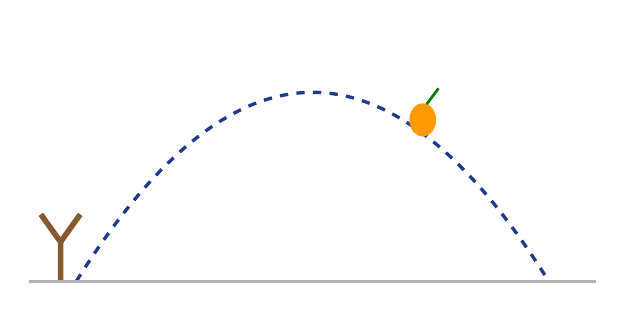
\begin{tikzpicture}
  \draw[azul, line width=1.2pt, dashed] (0,0) .. controls (2,3.2) and (4,3.2) .. (6,0);
  \fill[orange!80!yellow] (4.4,2.05) ellipse (0.17 and 0.21);
  \draw[green!50!black, line width=1pt] (4.45,2.25) -- (4.6,2.45);
  \draw[brown!70!black, line width=2pt] (-0.2,0) -- (-0.2,0.5) -- (-0.45,0.85);
  \draw[brown!70!black, line width=2pt] (-0.2,0.5) -- (0.05,0.85);
  \draw[gray!60, line width=1pt] (-0.6,0) -- (6.6,0);
\end{tikzpicture}
\par\vspace{0.8cm}
{\fontsize{30}{36}\selectfont\bfseries\color{azul} CinemaLab 2.0\par}
\vspace{6pt}
{\Large Resolvedor, Modo clase y juego de cinemática\par}
\vspace{4pt}
{\large Motor de física en Rust · API en Node.js · Interfaz en React\par}
\vspace{1.2cm}
{\large\bfseries Informe técnico\par}
\vfill
\begin{tabular}{ll}
\textbf{Integrantes:} & Dennis Ariel Avila Fuentes (AF23013) \\
 & \pend{Nombre del integrante 2 (carnet)} \\
 & \pend{Nombre del integrante 3 (carnet)} \\[6pt]
\textbf{Docente:} & \pend{Nombre del docente} \\
\textbf{Grupo:} & \pend{Grupo de clase} \\
\textbf{Fecha:} & Noviembre de 2026 \\
\end{tabular}
\vspace{1cm}
\end{titlepage}

\tableofcontents
\clearpage

% ================================================================ 1
\section{Introducción}

La cinemática estudia cómo se mueven los cuerpos sin preguntarse por qué se mueven. Es el primer tema de Mecánica Clásica y la base de todo lo que sigue. Al resolver ejercicios, el estudiante suele conocer las fórmulas, pero le cuesta decidir \emph{cuál} usar, despejarla e interpretar el resultado. Además, casi nunca ve el movimiento que está calculando.

Este proyecto presenta \textbf{CinemaLab 2.0}, una aplicación web con tres partes:

\begin{enumerate}
  \item Un \textbf{resolvedor paso a paso} de ejercicios de MRU, MRUA y lanzamiento parabólico. El usuario escribe los datos del enunciado y el programa elige la ecuación, la despeja, sustituye los valores y verifica que el resultado tenga sentido físico. Después anima el movimiento y dibuja sus gráficas.
  \item Un \textbf{Modo clase} que explica cada tema escena por escena, como una presentación. Cada escena trae la animación sincronizada, las fórmulas y narración por voz. Primero explica la teoría y luego el ejercicio del propio usuario.
  \item \textbf{``La hondilla''}, un juego de tiro parabólico ambientado en El Salvador, con tres modos: botar latas, bajar mangos de un palo y ``hondillazos'' entre dos amigos. Después de cada tiro, el juego explica la trayectoria y deduce el tiro perfecto.
\end{enumerate}

Toda la física está en un \textbf{motor escrito en Rust}. Una \textbf{API en Node.js} lo expone a una \textbf{interfaz en React}. Este informe describe los fundamentos físicos, los modelos matemáticos, la arquitectura, las funcionalidades y las pruebas del sistema.

% ================================================================ 2
\section{Descripción general del proyecto}

CinemaLab 2.0 es una aplicación web cliente–servidor organizada en tres pestañas, una por tema: MRU, MRUA y Parabólico. Cada pestaña tiene dos secciones, \emph{Resolver ejercicio} y \emph{Modo clase}. El parabólico agrega una tercera sección, el juego \emph{La hondilla}.

El flujo de una consulta es siempre el mismo:
\begin{enumerate}
  \item La interfaz (React) envía los datos del usuario a la API en formato JSON.
  \item La API (Node.js) valida los datos con esquemas de \texttt{zod} y llama al motor.
  \item El motor (Rust) resuelve el problema y genera la explicación paso a paso, la simulación, el guion del Modo clase o el resultado de un tiro.
  \item La interfaz recibe el resultado y lo muestra: fórmulas renderizadas con KaTeX, animaciones y gráficas en Canvas.
\end{enumerate}

La interfaz \textbf{no hace cálculos físicos}: dibuja y anima los datos que calcula el motor. Así, los resultados que se ven siempre son los que se probaron.

\begin{figure}[H]
  \centering
  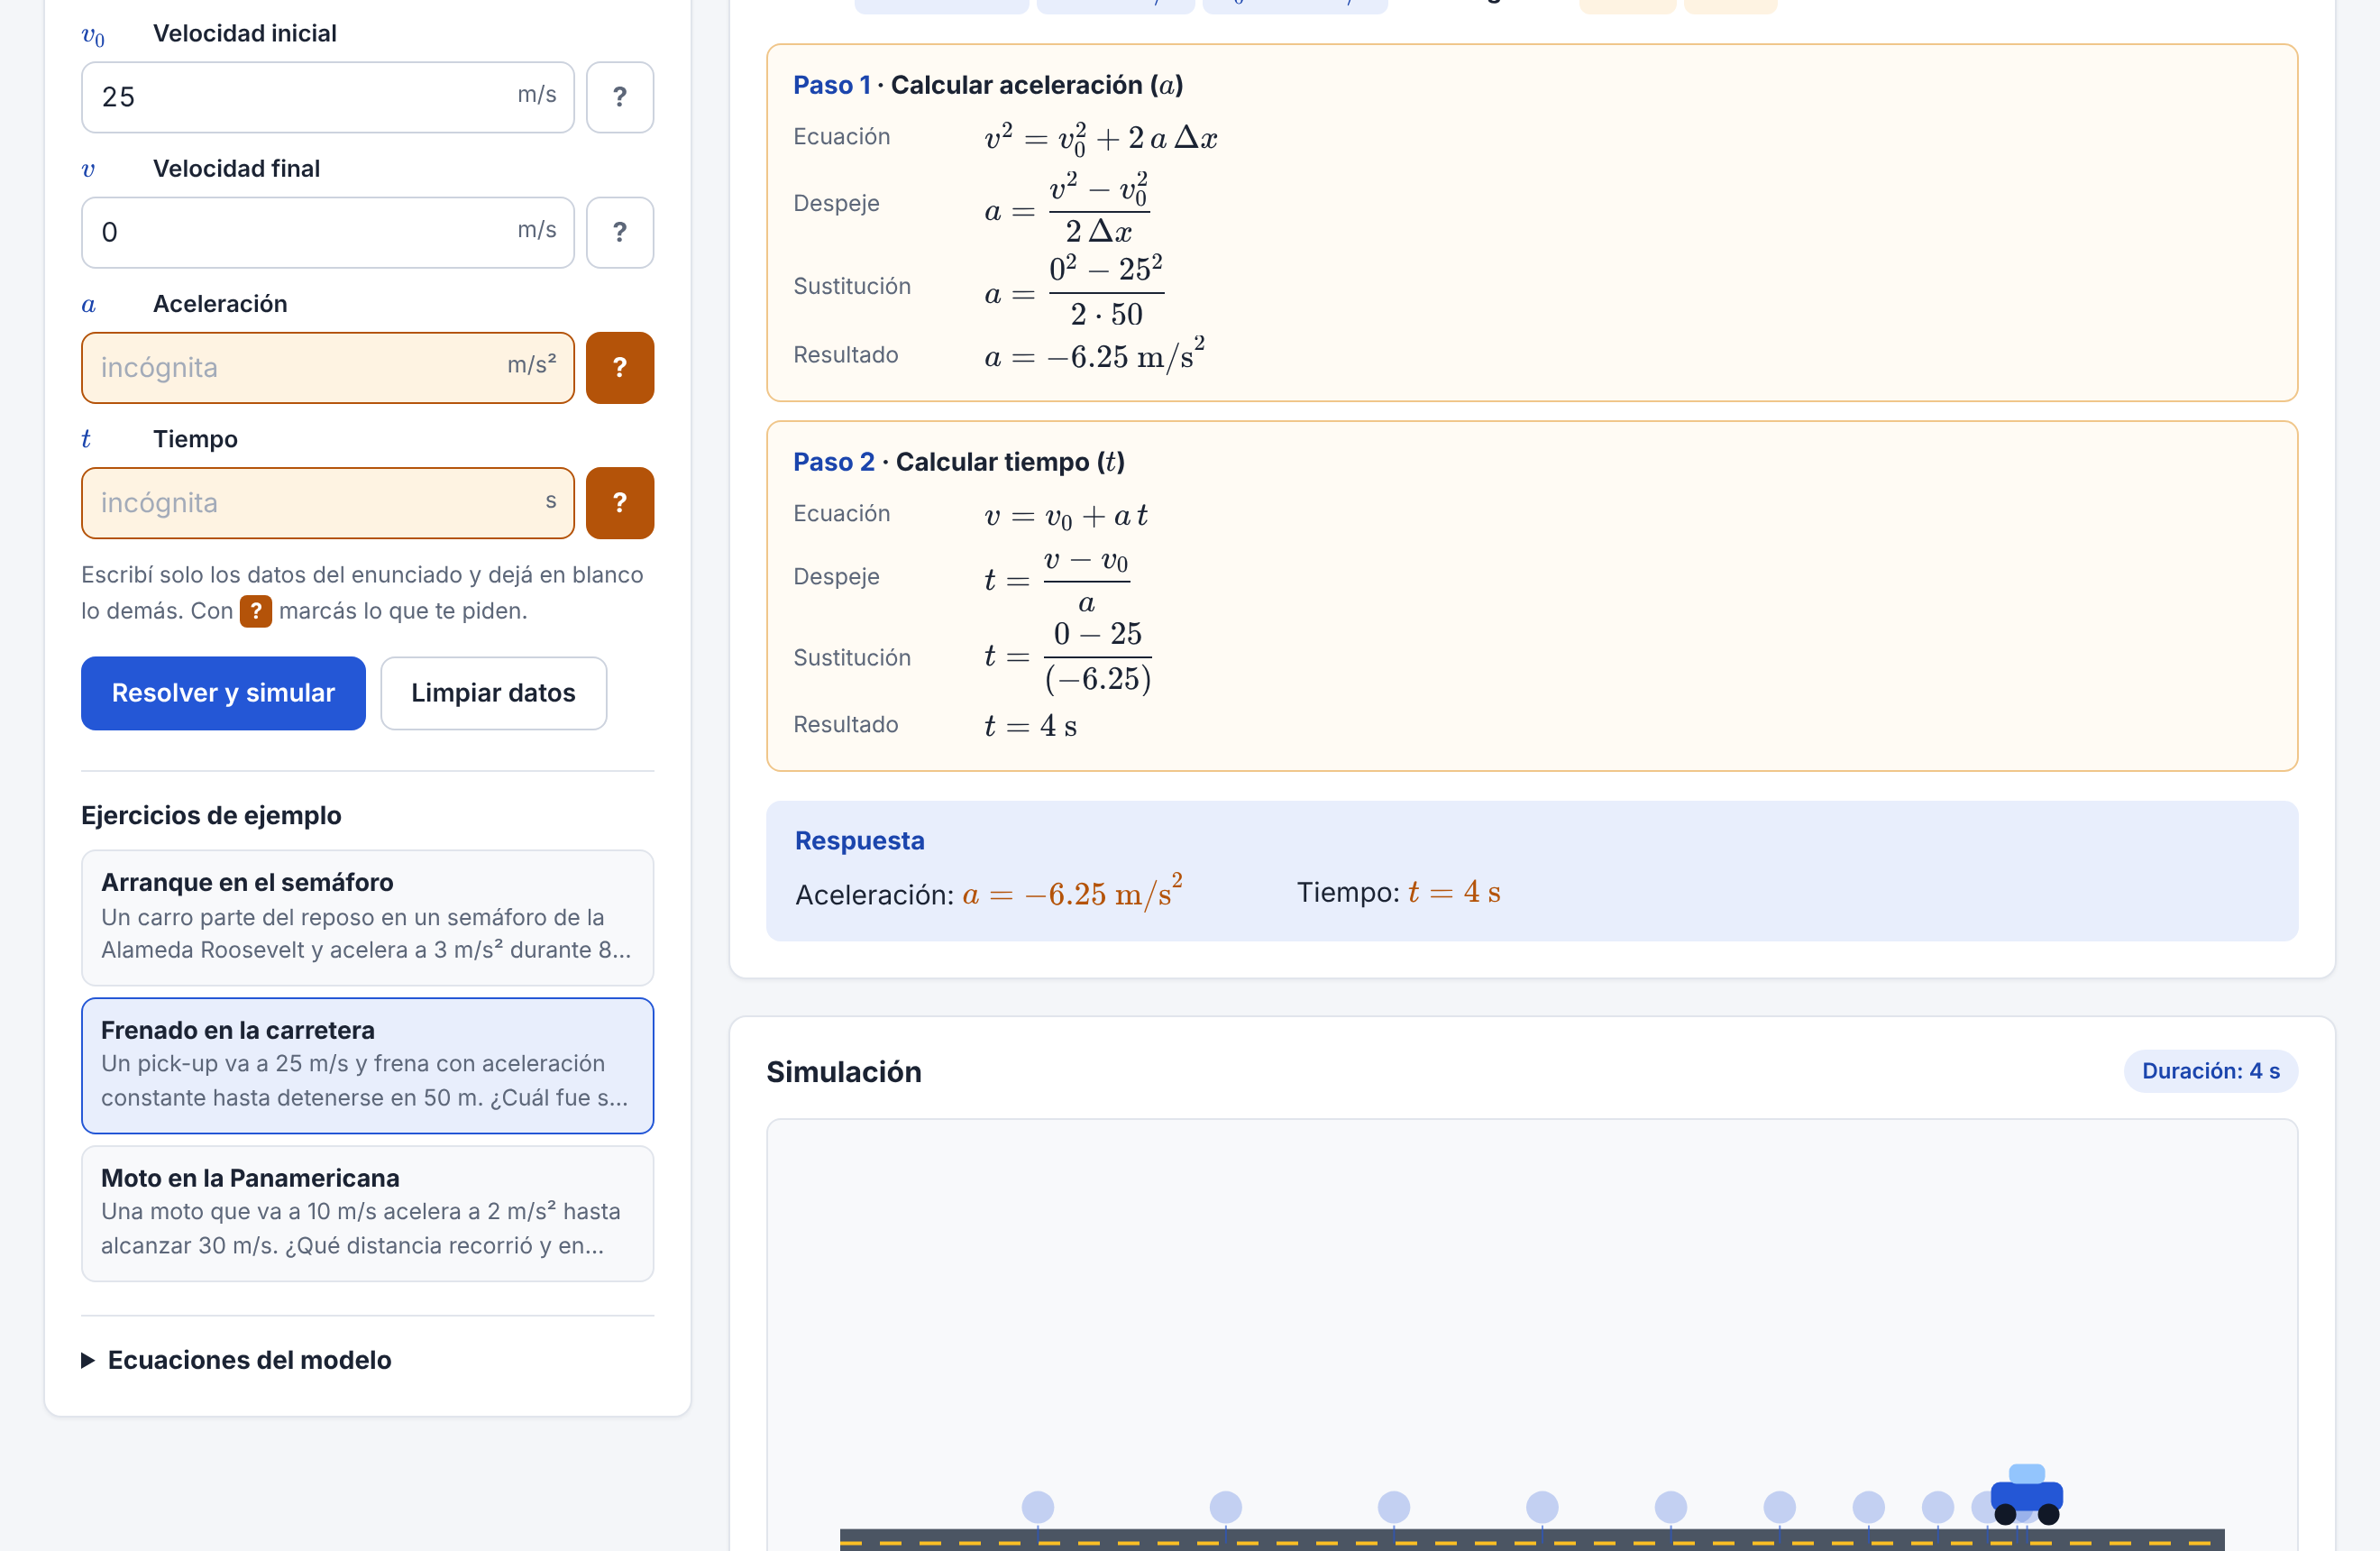
\includegraphics[width=\linewidth]{img/general.png}
  \caption{Resolvedor de MRUA con el ejercicio ``Frenado en la carretera'': solución paso a paso, simulación y gráficas.}
\end{figure}

% ================================================================ 3
\section{Objetivos}

\subsection{Objetivo general}

Desarrollar una aplicación web, con una arquitectura en capas (motor en Rust, API en Node.js e interfaz en React), que resuelva y explique paso a paso ejercicios de MRU, MRUA y lanzamiento parabólico, los simule y refuerce el aprendizaje del tiro parabólico con un juego ambientado en El Salvador.

\subsection{Objetivos específicos}

\begin{itemize}
  \item Implementar en Rust los modelos del MRU, el MRUA y el lanzamiento parabólico, con cada ecuación capaz de despejar cualquiera de sus variables.
  \item Diseñar un motor que elija las ecuaciones automáticamente y detecte datos insuficientes, datos inconsistentes y resultados sin sentido físico.
  \item Generar desde el motor el guion del Modo clase: narración, fórmulas y capas visuales de cada escena.
  \item Programar la física del juego (trayectoria, choques, latas, mangos y caída libre) y la deducción del tiro perfecto.
  \item Exponer el motor mediante una API REST en Node.js con validación de entradas y contratos compartidos.
  \item Construir una interfaz en React con animaciones, gráficas sincronizadas, fórmulas en notación matemática y diseño adaptable a teléfonos.
  \item Validar el sistema con pruebas automáticas en cada capa.
\end{itemize}

% ================================================================ 4
\section{Alcance}

\textbf{Incluye:}
\begin{itemize}
  \item MRU, MRUA y lanzamiento parabólico desde el suelo o desde una altura $h_0$.
  \item Resolución de cualquier variable de cada modelo, con todos los pasos, notas sobre raíces dobles y ambigüedad de signo, y avisos de datos inconsistentes o imposibles.
  \item Simulación con marcas estroboscópicas, vectores de velocidad y ``rayos X'' (las sombras del móvil sobre cada eje). Gráficas $x$–$t$, $v$–$t$, $a$–$t$ y la trayectoria. Tabla de valores y exportación a CSV.
  \item Modo clase para los tres temas: 7 a 15 escenas, narración por voz opcional y avance automático.
  \item Juego con 10 escenarios: 5 de latas, 3 de mangos y 2 duelos para dos jugadores.
\end{itemize}

\textbf{No incluye:}
\begin{itemize}
  \item Resistencia del aire, viento ni rotación de los cuerpos.
  \item Movimiento circular, movimiento relativo y dinámica.
  \item Lectura automática de enunciados escritos: los datos se ingresan en el formulario.
\end{itemize}

% ================================================================ 5
\section{Tecnologías utilizadas}

\begin{table}[H]
\centering
\small
\begin{tabularx}{\linewidth}{@{}llX@{}}
\toprule
\textbf{Capa} & \textbf{Tecnología} & \textbf{Uso} \\
\midrule
Motor & Rust (edición 2021) & Modelos físicos, resolvedor, simulación, lecciones y juego. Se eligió por su rendimiento y su seguridad de memoria, y porque obliga a manejar todos los errores. \\
 & serde / serde\_json & Conversión de las estructuras de Rust a JSON y de JSON a Rust. \\
Puente & napi-rs & Compila el motor como módulo nativo de Node.js (\texttt{fisica.node}). \\
API & Node.js 22 + TypeScript & Servidor de la aplicación. \\
 & Fastify 5 & Rutas REST y entrega de la web compilada. \\
 & zod & Validación de las entradas y contratos compartidos con la web. \\
Interfaz & React 18 + TypeScript & Componentes de la interfaz. \\
 & Vite 6 & Servidor de desarrollo y compilación de la web. \\
 & KaTeX & Fórmulas en notación matemática, escritas en \LaTeX{} por el motor. \\
 & Canvas 2D y Web Speech API & Animaciones, gráficas, juego y narración por voz. \\
Herramientas & pnpm (workspaces) y cargo & Monorepo: dependencias y compilación de cada parte. \\
 & cargo test, Vitest, Playwright & Pruebas del motor, de la API, de la web y de punta a punta. \\
 & Docker, Render & Publicación del sistema completo. \\
\bottomrule
\end{tabularx}
\caption{Tecnologías por capa.}
\end{table}

% ================================================================ 6
\section{Fundamentos teóricos}

\textbf{Posición, velocidad y aceleración.} La posición $x(t)$ indica dónde está el móvil en cada instante. La velocidad es la rapidez con que cambia la posición, $v = dx/dt$, y la aceleración es la rapidez con que cambia la velocidad, $a = dv/dt$.

\textbf{MRU.} La velocidad es constante y la aceleración es cero. El móvil recorre distancias iguales en tiempos iguales: la gráfica $x$–$t$ es una recta y la $v$–$t$ es horizontal.

\textbf{MRUA.} La aceleración es constante, así que la velocidad cambia lo mismo cada segundo: la gráfica $v$–$t$ es una recta y la $x$–$t$ es una parábola. El área bajo la gráfica $v$–$t$ es el desplazamiento.

\textbf{Lanzamiento parabólico.} Según el principio de independencia de los movimientos, el movimiento horizontal y el vertical ocurren al mismo tiempo sin afectarse. En $x$ no hay aceleración (MRU) y en $y$ la gravedad produce una aceleración constante $-g$ (MRUA). Al combinarse, la trayectoria es una parábola.

\textbf{Un solo modelo general.} Los tres movimientos son casos de un móvil con aceleración constante en el plano:
\[
  x(t) = x_0 + v_{x0}\,t + \tfrac12 a_x t^2, \qquad y(t) = y_0 + v_{y0}\,t + \tfrac12 a_y t^2 .
\]
El MRU tiene $a_x = 0$, el MRUA tiene $a_x = a$ y el parabólico tiene $a_y = -g$. El motor aprovecha este hecho: un mismo tipo \texttt{Movimiento} simula los tres casos.

\subsection{Convenciones físicas}

\begin{itemize}
  \item Unidades del Sistema Internacional (m, s, m/s, m/s$^2$); los ángulos van en grados.
  \item Eje $x$ positivo hacia la derecha y eje $y$ positivo hacia arriba.
  \item En el parabólico, el origen está en el suelo, bajo el punto de lanzamiento: el proyectil sale de $(0, h_0)$.
  \item $g = 9.81$ m/s$^2$ hacia $-y$. Se puede cambiar en el formulario.
  \item El ángulo $\theta$ se mide desde la horizontal, con $0^\circ \le \theta \le 90^\circ$.
  \item Se desprecia la resistencia del aire y los cuerpos se tratan como partículas.
  \item Ningún tiempo puede ser negativo: un despeje que dé $t < 0$ se descarta y se avisa.
\end{itemize}

% ================================================================ 7
\section{Ecuaciones y modelos matemáticos}

\subsection{Movimiento Rectilíneo Uniforme (MRU)}

\begin{equation}
  \Delta x = v\,t \qquad\Longrightarrow\qquad v = \frac{\Delta x}{t}, \qquad t = \frac{\Delta x}{v}
\end{equation}
Con dos de las tres variables se obtiene la tercera.

\subsection{Movimiento Rectilíneo Uniformemente Acelerado (MRUA)}

\begin{align}
  v &= v_0 + a\,t & &(\text{no tiene } \Delta x) \label{eq:m1}\\
  \Delta x &= v_0\,t + \tfrac12 a\,t^2 & &(\text{no tiene } v) \label{eq:m2}\\
  v^2 &= v_0^2 + 2a\,\Delta x & &(\text{no tiene } t) \label{eq:m3}\\
  \Delta x &= \tfrac12 (v_0 + v)\,t & &(\text{no tiene } a) \label{eq:m4}
\end{align}
Cada ecuación deja fuera una de las cinco variables. Por eso, con tres datos siempre hay una ecuación con una sola incógnita. El Modo clase enseña esta misma regla: \emph{usar la ecuación que no tiene la variable que ni te dan ni te piden}.

Hay despejes que necesitan cuidado. El tiempo en \eqref{eq:m2} sale de una cuadrática:
\[
  \tfrac12 a\,t^2 + v_0\,t - \Delta x = 0 \;\Rightarrow\; t = \frac{-v_0 \pm \sqrt{v_0^2 + 2a\Delta x}}{a}.
\]
Se toma la menor raíz positiva, y si hay otra, se informa. Si el discriminante es negativo, el móvil nunca llega a esa posición. Despejar $v$ o $v_0$ de \eqref{eq:m3} deja un signo $\pm$; se toma el sentido del movimiento y se explica la suposición en una nota.

\subsection{Lanzamiento parabólico}

\begin{gather}
  v_{0x} = v_0\cos\theta, \qquad v_{0y} = v_0\sen\theta \\
  x(t) = v_{0x}\,t, \qquad y(t) = h_0 + v_{0y}\,t - \tfrac12 g\,t^2, \qquad v_y = v_{0y} - g\,t \\
  t_s = \frac{v_{0y}}{g}, \qquad h_{\max} = h_0 + \frac{v_{0y}^2}{2g} \\
  t_v = \frac{v_{0y} + \sqrt{v_{0y}^2 + 2g\,h_0}}{g}, \qquad R = v_{0x}\,t_v \\
  R = \frac{v_0^2 \sen 2\theta}{g} \quad (\text{solo si } h_0 = 0)
\end{gather}
La última fórmula solo se usa cuando el proyectil sale y cae al mismo nivel. Muestra que el alcance máximo se logra con $45^\circ$ y que dos ángulos complementarios dan el mismo alcance. Cuando se pide $\theta$ a partir de $R$, el programa muestra las dos soluciones.

\subsection{Ecuación de la trayectoria}

Despejando $t = x/(v_0\cos\theta)$ del movimiento horizontal y sustituyendo en $y(t)$:
\begin{equation}
  \boxed{\,y(x) = h_0 + x\tan\theta - \frac{g\,x^2}{2\,v_0^2\cos^2\theta}\,}
  \label{eq:tray}
\end{equation}

\subsection{Tiro perfecto en el juego}

Si el objetivo está a una distancia horizontal $d$ de la hondilla y a una altura $y$, y la hondilla está a $y_0$, se pone ese punto en \eqref{eq:tray} y se despeja la rapidez:
\begin{equation}
  \boxed{\,v_0 = \frac{d}{\cos\theta}\sqrt{\frac{g}{2\,(y_0 + d\tan\theta - y)}}\,}
  \label{eq:perfecto}
\end{equation}
La raíz existe solo si $y_0 + d\tan\theta > y$, es decir, si la línea de lanzamiento apunta por encima del objetivo. La fórmula no considera obstáculos. Por eso el motor simula el tiro calculado y, si choca con un muro o un tronco, busca el ángulo más cercano que sí llegue con una rapidez entre 5 y 35 m/s.

\subsection{Caída libre del mango}

Cuando la piedra golpea un mango, el mango se suelta desde el reposo a una altura $h$. Su movimiento es un MRUA con $v_0 = 0$ y $a = -g$:
\begin{equation}
  t = \sqrt{\frac{2h}{g}}, \qquad v = \sqrt{2\,g\,h}.
\end{equation}
El Modo clase usa la misma idea en la escena ``El mango que se cae del palo''. Un mango que se suelta a la altura máxima, justo cuando pasa la piedra, llega al suelo al mismo tiempo que ella. La razón es que, desde ese punto, los dos tienen el mismo movimiento vertical: $t_v - t_s = \sqrt{2h_{\max}/g}$.

% ================================================================ 8
\section{Arquitectura del software}

\subsection{Capas y flujo de datos}

El sistema es un \textbf{monorepo} con un \emph{workspace} de pnpm (Node.js) y otro de cargo (Rust). Tiene cuatro capas con responsabilidades separadas:

\begin{figure}[H]
\centering
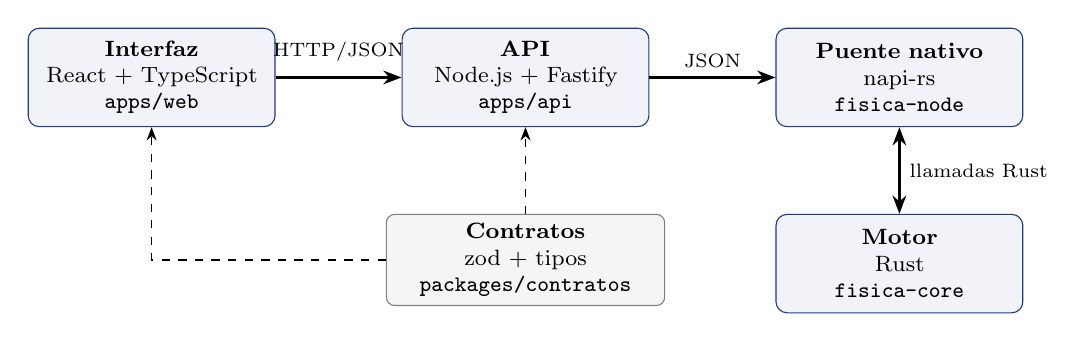
\begin{tikzpicture}[
  node distance=0.5cm and 0.8cm,
  capa/.style={draw=azul, rounded corners=4pt, fill=azul!6, align=center, minimum height=1.25cm, text width=2.9cm, font=\footnotesize},
  dato/.style={draw=gray, rounded corners=3pt, fill=gray!8, align=center, minimum height=0.9cm, text width=3.3cm, font=\footnotesize},
  >=Stealth]
  \node[capa] (web) {\textbf{Interfaz}\\React + TypeScript\\\texttt{apps/web}};
  \node[capa, right=1.6cm of web] (api) {\textbf{API}\\Node.js + Fastify\\\texttt{apps/api}};
  \node[capa, right=1.6cm of api] (puente) {\textbf{Puente nativo}\\napi-rs\\\texttt{fisica-node}};
  \node[capa, below=1.1cm of puente] (motor) {\textbf{Motor}\\Rust\\\texttt{fisica-core}};
  \node[dato, below=1.1cm of api] (contratos) {\textbf{Contratos}\\zod + tipos\\\texttt{packages/contratos}};
  \draw[->, thick] (web) -- node[above,font=\scriptsize,yshift=2pt]{HTTP/JSON} (api);
  \draw[->, thick] (api) -- node[above,font=\scriptsize]{JSON} (puente);
  \draw[<->, thick] (puente) -- node[right,font=\scriptsize]{llamadas Rust} (motor);
  \draw[->, dashed] (contratos) -- (api);
  \draw[->, dashed] (contratos) -| (web);
\end{tikzpicture}
\caption{Capas del sistema y flujo de datos.}
\end{figure}

\begin{enumerate}
  \item \textbf{Motor (\texttt{fisica-core}, Rust)}: es el dominio puro. No sabe nada de HTTP ni del navegador. Recibe estructuras y devuelve estructuras serializables. Contiene los modelos, el resolvedor, la simulación, los guiones del Modo clase y la física del juego.
  \item \textbf{Puente (\texttt{fisica-node}, napi-rs)}: compila el motor como un módulo nativo que Node.js carga con \texttt{require}. Cada función recibe y devuelve JSON, así que el contrato es simple y estable.
  \item \textbf{API (\texttt{apps/api}, Fastify)}: valida cada petición con \texttt{zod} y responde 400 si los datos están mal formados, 422 si el motor rechaza la petición y 500 ante errores internos. Llama al motor y sirve la web compilada.
  \item \textbf{Interfaz (\texttt{apps/web}, React)}: muestra la información y anima. No evalúa ecuaciones: \textbf{interpola} las muestras que calculó el motor (601 por simulación y 60 por segundo en el juego).
\end{enumerate}

\subsection{Responsabilidades de los módulos principales}

\begin{table}[H]
\centering
\small
\begin{tabularx}{\linewidth}{@{}lX@{}}
\toprule
\textbf{Módulo} & \textbf{Responsabilidad} \\
\midrule
\texttt{fisica-core/src/modelo.rs} & Tipos del dominio: \texttt{Variable}, \texttt{Ecuacion} (con sus despejes en \LaTeX), \texttt{Modelo}, \texttt{Despeje}. \\
\texttt{fisica-core/src/modelos/} & MRU, MRUA y parabólico: variables, ecuaciones y ejercicios de ejemplo con contexto salvadoreño. \\
\texttt{fisica-core/src/solver.rs} & Motor de resolución paso a paso, validación de rangos y verificación de consistencia. \\
\texttt{fisica-core/src/movimiento.rs} & Movimiento con aceleración constante, muestreo y eventos (punto más alto, detención). \\
\texttt{fisica-core/src/leccion.rs} & Guiones del Modo clase: escenas con narración, fórmulas, capas visuales y tramo de tiempo. \\
\texttt{fisica-core/src/juego/} & Escenarios, trayectoria y choques del tiro, análisis con frases salvadoreñas y tiro perfecto. \\
\texttt{fisica-core/src/api.rs} & Funciones JSON $\to$ JSON: la única puerta de entrada al motor. \\
\texttt{fisica-node/src/lib.rs} & Exporta esas funciones a Node.js con \texttt{\#[napi]}. \\
\texttt{apps/api/src/app.ts} & Construye la aplicación Fastify, el manejo de errores y la entrega de la web. \\
\texttt{apps/api/src/motor.ts} & Acceso tipado al módulo nativo y caché de modelos y escenarios. \\
\texttt{apps/web/src/componentes/} & \texttt{resolvedor/}, \texttt{simulacion/}, \texttt{graficas/}, \texttt{clase/} y \texttt{juego/}. \\
\texttt{packages/contratos} & Esquemas \texttt{zod} de entrada y tipos de salida que reflejan las estructuras de Rust. \\
\bottomrule
\end{tabularx}
\caption{Módulos principales.}
\end{table}

\subsection{Motor de resolución paso a paso}

Cada ecuación sabe despejar cada una de sus variables. Cada despeje tiene una \emph{prioridad}: 1 si es lineal, 2 si lleva raíz o cuadrática y 3 si tiene ambigüedad de signo. El algoritmo imita a un estudiante:

\begin{lstlisting}[caption={Algoritmo del resolvedor (\texttt{solver.rs}).}]
conocidos <- datos del usuario (+ g = 9.81 y h0 = 0 si no se dan)
repetir:
  candidatas <- ecuaciones con exactamente UNA variable desconocida
  si no hay candidatas: terminar
  elegir el despeje de menor prioridad          // primero lo más sencillo
  despejar, sustituir y calcular (en LaTeX)
  si no tiene sentido físico (t < 0, raíz negativa): avisar y descartar
  si no: guardar el paso y marcar la variable como conocida
marcar los pasos necesarios para las incógnitas pedidas (recorrido hacia atrás)
verificar que todas las ecuaciones se cumplan (tolerancia del 1 %)
\end{lstlisting}

Así se define una ecuación en Rust: cada despeje es una función que devuelve el valor y la sustitución escrita en \LaTeX.

\begin{lstlisting}[language=Rust,caption={Ecuación $v = v_0 + a\,t$ en \texttt{mrua.rs} (resumida).}]
Ecuacion {
    id: "mrua1",
    latex: "v = v_0 + a\\,t",
    vars: &["v", "v0", "a", "t"],
    despejes: vec![
        FormaDespejada { var: "t", latex: "t = \\dfrac{v - v_0}{a}", prioridad: 1, f: |v| {
            if !nz(v.g("a")) { return Despeje::NoAplica; }   // no dividir entre cero
            Despeje::ok((v.g("v") - v.g("v0")) / v.g("a"), format!("t = ...", ...))
        }},
        // ... despejes de v, v0 y a
    ],
    ..
}
\end{lstlisting}

\subsection{Contratos y validación}

Los datos se validan en los dos extremos. La API usa \texttt{zod}: por ejemplo, el ángulo del juego debe estar entre $5^\circ$ y $85^\circ$. El motor usa \texttt{serde} y además revisa los rangos físicos de cada variable. El paquete \texttt{@cinemalab/contratos} define los tipos de las respuestas para que la API y la web usen exactamente la misma forma de datos que produce Rust.

% ================================================================ 9
\section{Estructura de archivos}

\begin{lstlisting}[caption={Estructura del repositorio.}]
cinemalab/
+-- Cargo.toml               workspace de Rust
+-- package.json             scripts: dev, build, test, start
+-- pnpm-workspace.yaml      workspace de pnpm
+-- Dockerfile, render.yaml  publicación
+-- crates/
|   +-- fisica-core/         motor (modelos, solver, movimiento, leccion, juego, api)
|   |   `-- tests/           pruebas de validación
|   `-- fisica-node/         puente napi -> fisica.node
+-- apps/
|   +-- api/                 Fastify (src/app.ts, src/motor.ts, src/rutas/, test/)
|   `-- web/                 React (src/componentes/, src/lib/, src/hooks/, test/)
+-- packages/
|   `-- contratos/           esquemas zod y tipos
`-- scripts/
    `-- compilar-nativo.mjs  compila el motor (Windows, macOS y Linux)
\end{lstlisting}

% ================================================================ 10
\section{Funcionalidades}

\subsection{Entrada de datos}

Cada variable tiene su campo, con el símbolo en notación matemática, el nombre y la unidad. El botón ``?'' marca una variable como incógnita. Se acepta coma o punto decimal. Los valores fuera de rango (tiempo negativo, ángulo mayor que $90^\circ$) se marcan en rojo, y los datos escritos se conservan al cambiar de pestaña. Cada tema trae tres ejercicios de ejemplo con contexto local: el microbús de la ruta, un pick-up que frena en la carretera, un cohete de pólvora en diciembre, una piedra lanzada desde un mirador del Cerro Verde.

\subsection{Resolución paso a paso}

Cada paso muestra la ecuación, el despeje, la sustitución con los números y el resultado. Cuando el usuario marca incógnitas, solo se muestran los pasos necesarios para llegar a ellas; los demás se pueden ver con un clic. También se avisa cuando los datos son inconsistentes o no tienen solución física (figura~\ref{fig:imposible}).

\begin{figure}[H]
  \centering
  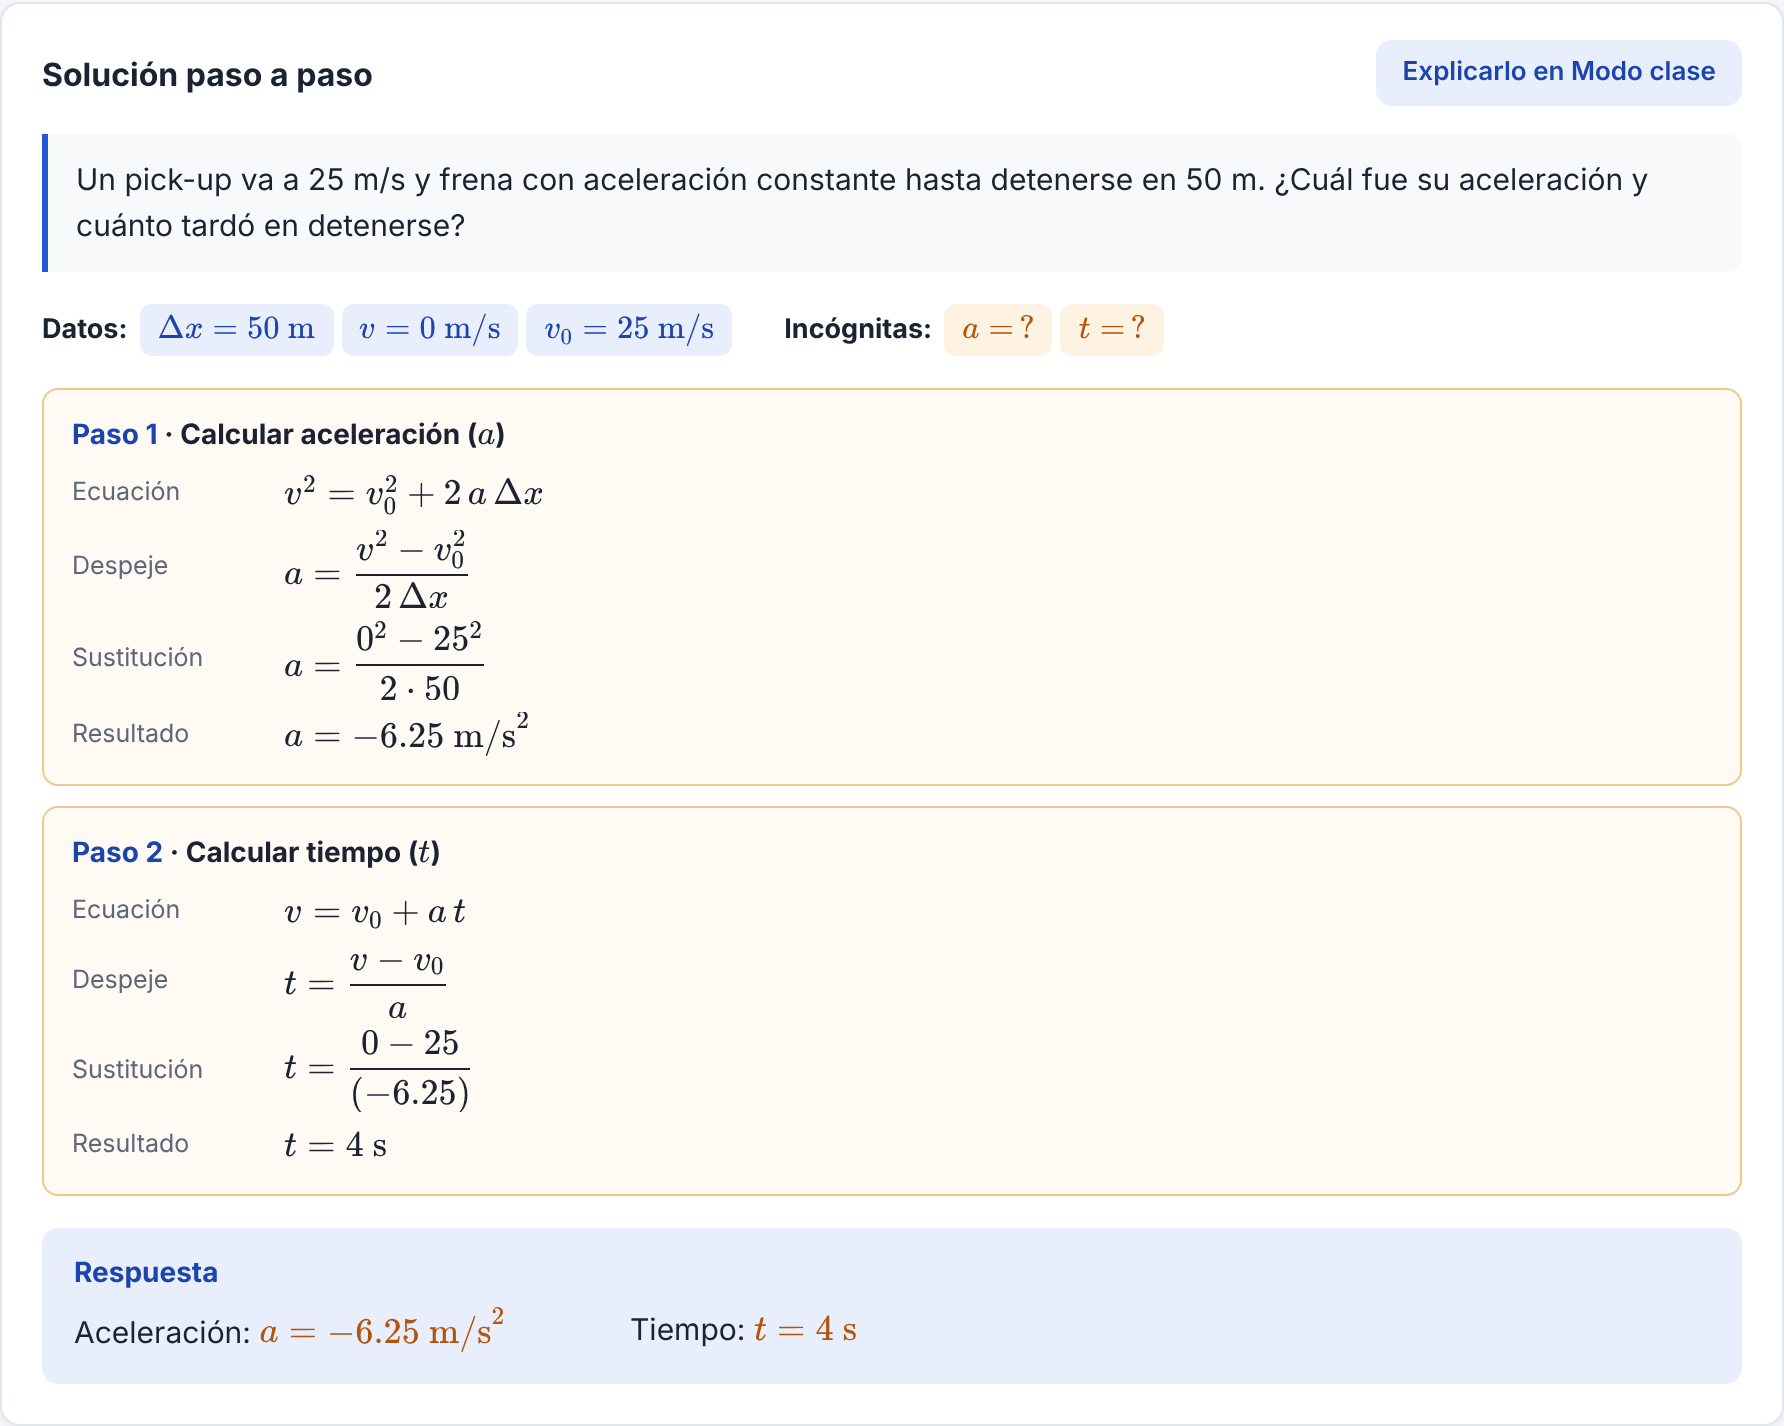
\includegraphics[width=0.8\linewidth]{img/solucion.png}
  \caption{Solución del frenado. El motor elige $v^2 = v_0^2 + 2a\Delta x$ para obtener $a$ (no tiene $t$) y luego $v = v_0 + at$ para obtener $t$.}
\end{figure}

\begin{figure}[H]
  \centering
  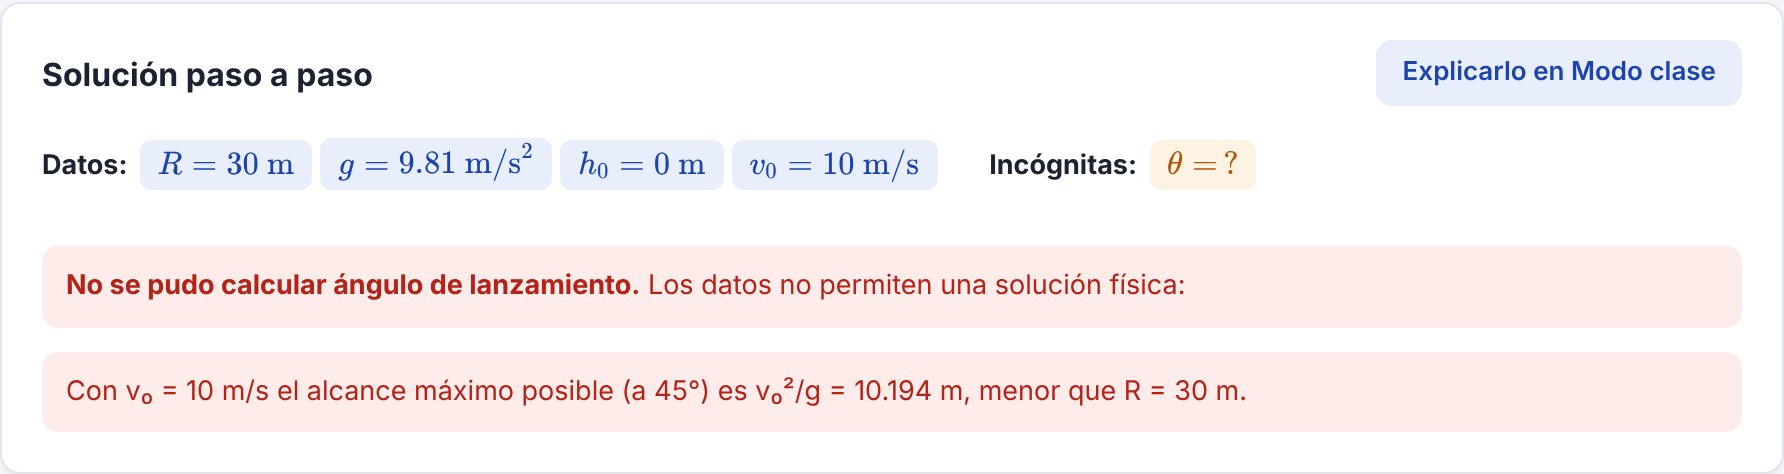
\includegraphics[width=0.7\linewidth]{img/aviso_imposible.png}
  \caption{Aviso de datos imposibles: con $v_0 = 10$ m/s no existe ángulo que dé un alcance de 30 m.}
  \label{fig:imposible}
\end{figure}

\subsection{Simulación y gráficas}

La animación muestra el móvil, los vectores de velocidad, las marcas estroboscópicas y, en el parabólico, la trayectoria y la altura máxima. Tiene controles para reproducir, pausar, recorrer la línea de tiempo y cambiar la velocidad, y muestra los valores instantáneos. En las gráficas, un cursor marca el mismo instante que la animación. También hay una tabla de valores y una opción para descargar los datos en CSV.

\begin{figure}[H]
  \centering
  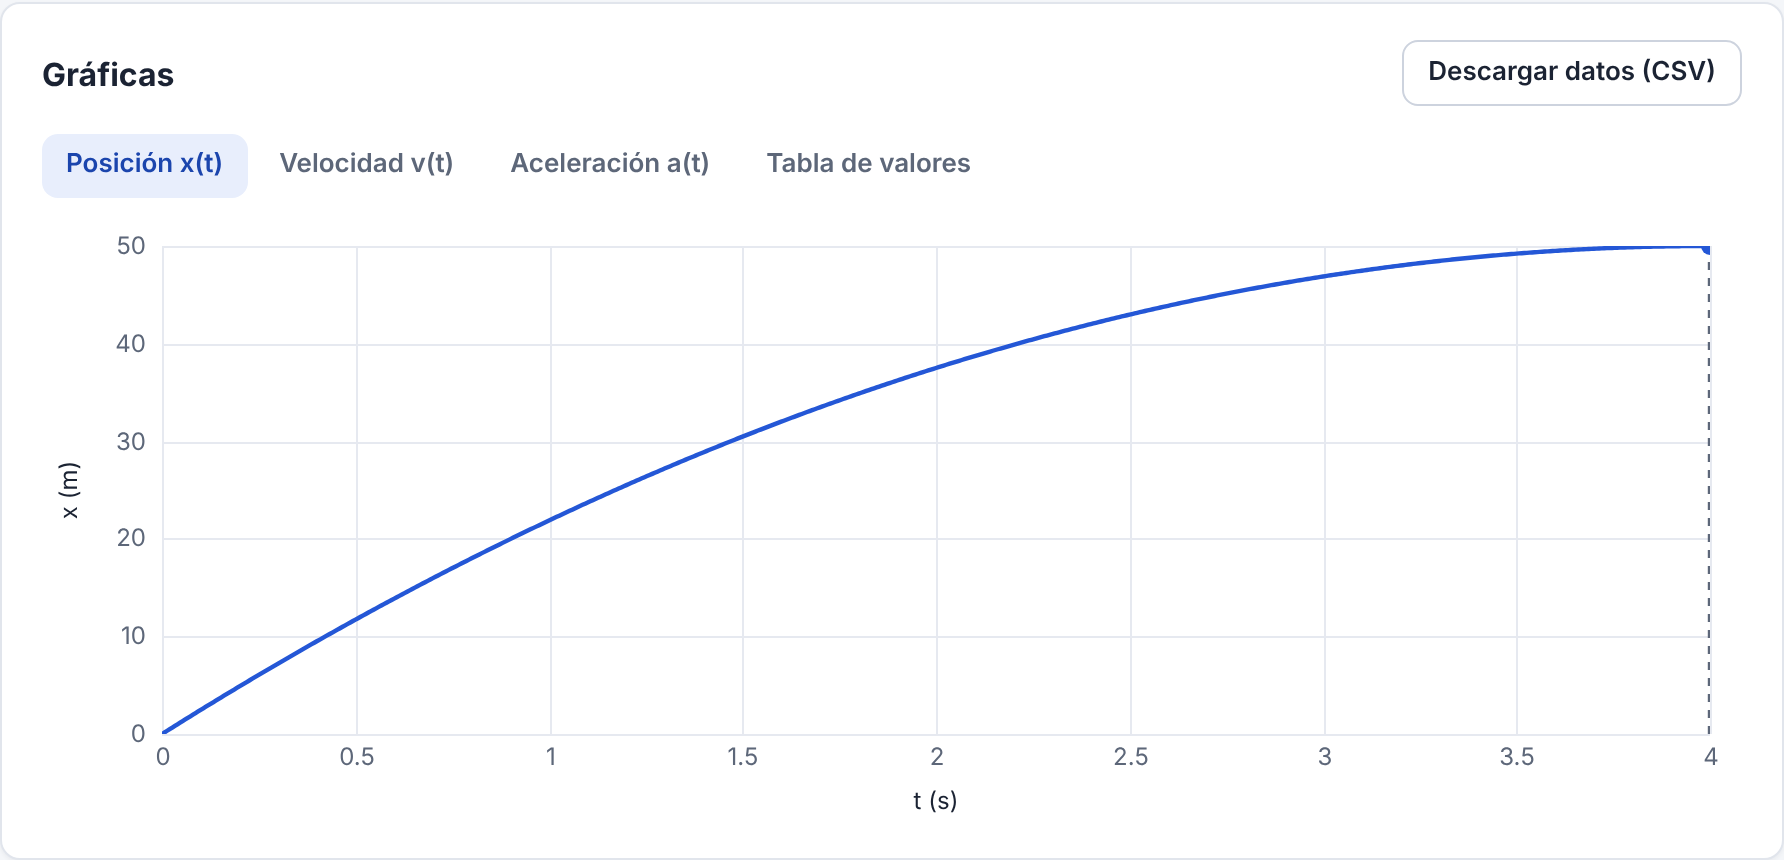
\includegraphics[width=0.75\linewidth]{img/graficas.png}
  \caption{Gráfica $x$–$t$ del frenado: una parábola que se aplana hasta que el carro se detiene.}
\end{figure}

\subsection{Modo clase}

El Modo clase reproduce un guion que genera el motor. Cada escena incluye un título, la narración (escrita para leerse en voz alta), las fórmulas, las capas visuales y el tramo de tiempo que se anima. La interfaz solo reproduce el guion: todos los números salen de Rust. Hay controles para ir a la escena anterior y a la siguiente, repetir una escena, activar la narración por voz y avanzar automáticamente. También se puede navegar con las flechas del teclado.

\begin{table}[H]
\centering
\small
\begin{tabularx}{\linewidth}{@{}lX@{}}
\toprule
\textbf{Tema} & \textbf{Escenas} \\
\midrule
MRU & Qué es · distancias iguales en tiempos iguales (con regla) · la ecuación · $x$–$t$ es recta · área bajo $v$–$t$ · tu ejercicio · resumen. \\
MRUA & Qué es · las marcas se separan o se juntan · $v$–$t$ con pendiente $a$ · $x$–$t$ es parábola · área = trapecio · las cuatro ecuaciones y cuál usar · el móvil se detiene · tu ejercicio · resumen. \\
Parabólico & Dos movimientos en uno (rayos X) · descomposición de $v_0$ · MRU en $x$ · MRUA en $y$ · punto más alto · tiempo de vuelo y alcance · el mango que se cae del palo · ecuación de la trayectoria · por qué $45^\circ$ · tu ejercicio · resumen. \\
\bottomrule
\end{tabularx}
\caption{Contenido del Modo clase.}
\end{table}

Desde el resolvedor, el botón \emph{Explicarlo en Modo clase} genera la clase con los datos del ejercicio del usuario. Si los datos no alcanzan para simular, se usa un ejemplo del tema.

\begin{figure}[H]
  \centering
  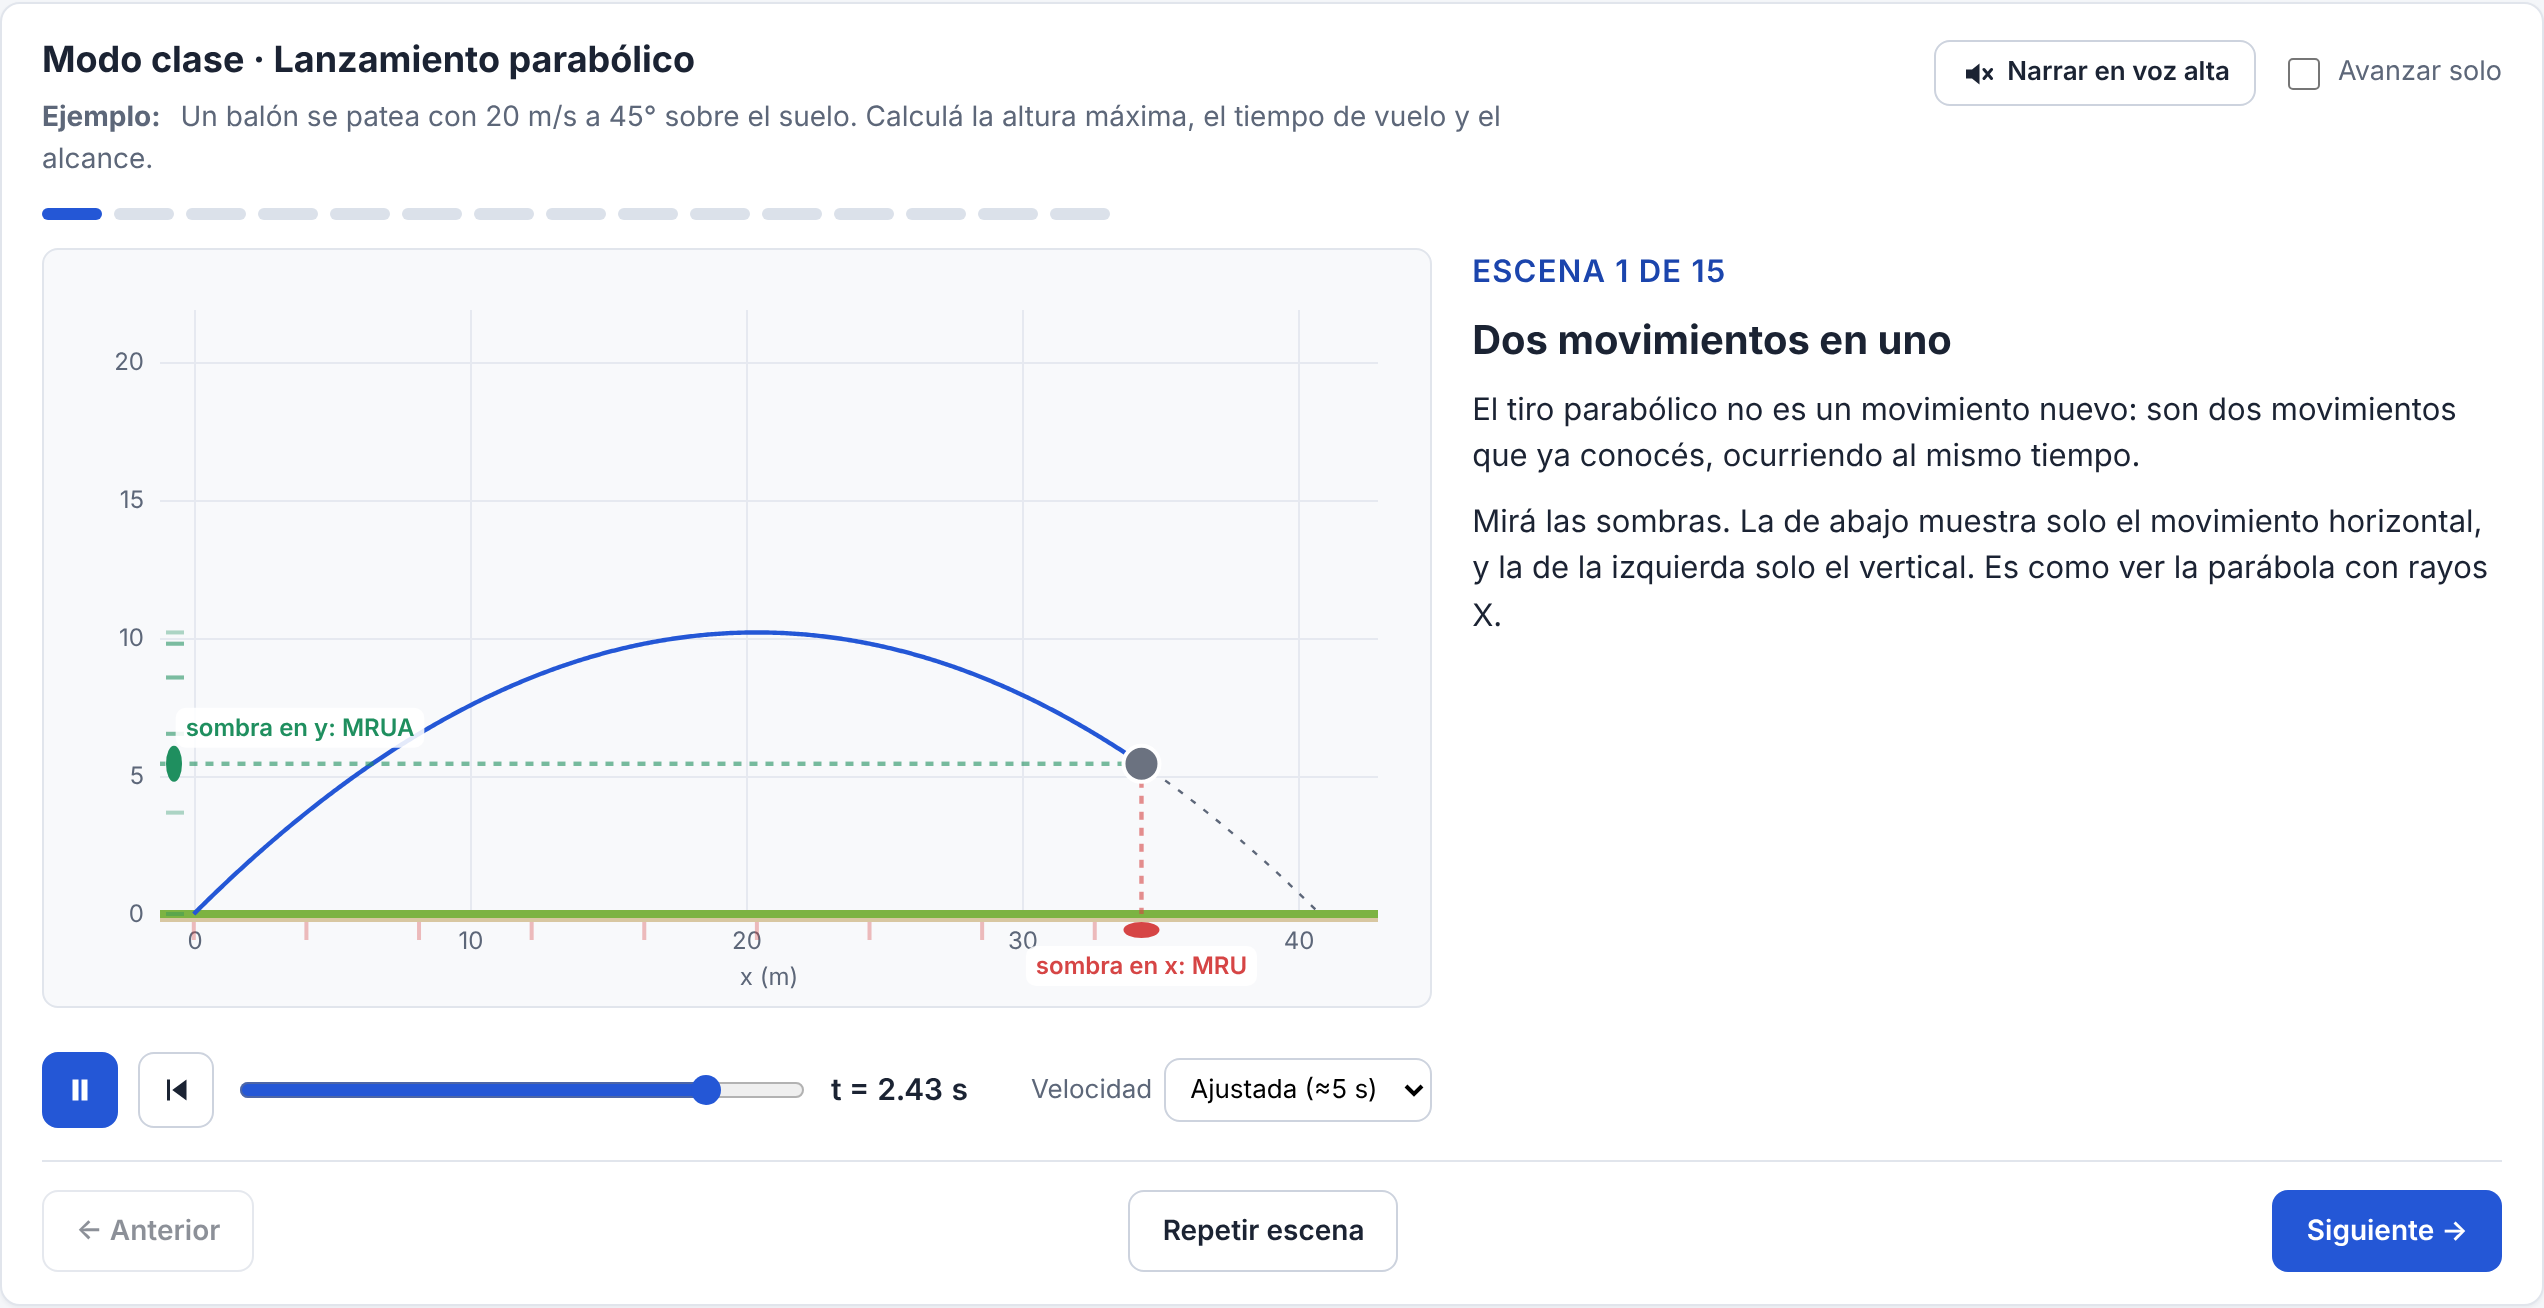
\includegraphics[width=0.49\linewidth]{img/clase_rayosx.png}\hfill
  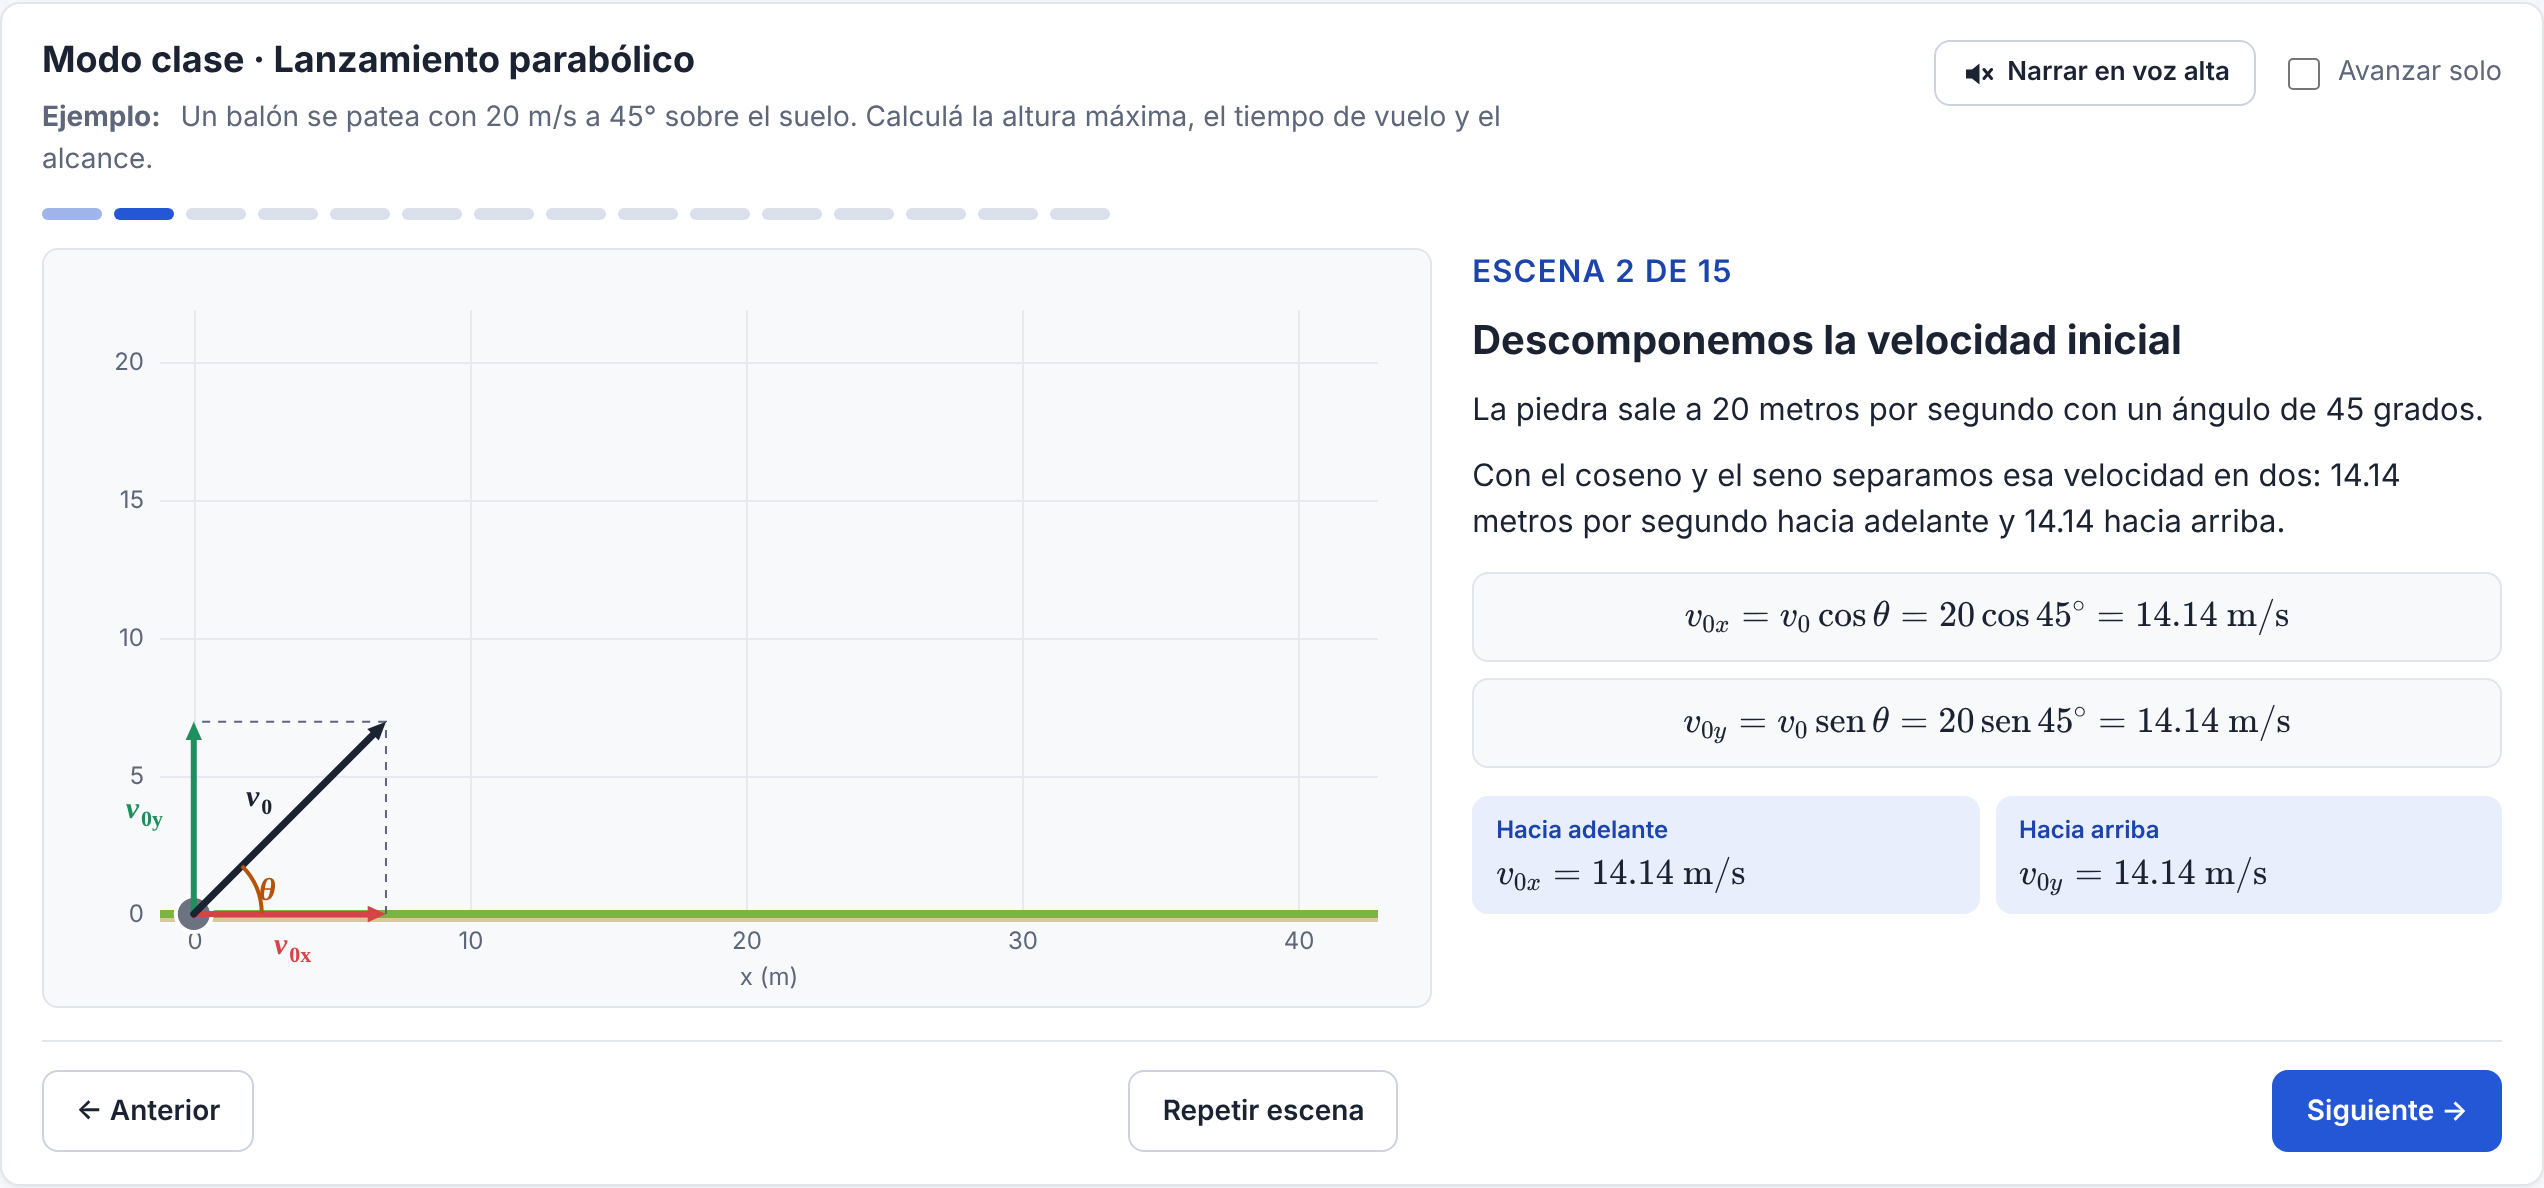
\includegraphics[width=0.49\linewidth]{img/clase_componentes.png}
  \caption{Modo clase del parabólico. Izquierda: ``rayos X'', la sombra en $x$ avanza pareja (MRU) y la sombra en $y$ sube y baja (MRUA). Derecha: descomposición de $v_0$ en sus componentes.}
\end{figure}

\begin{figure}[H]
  \centering
  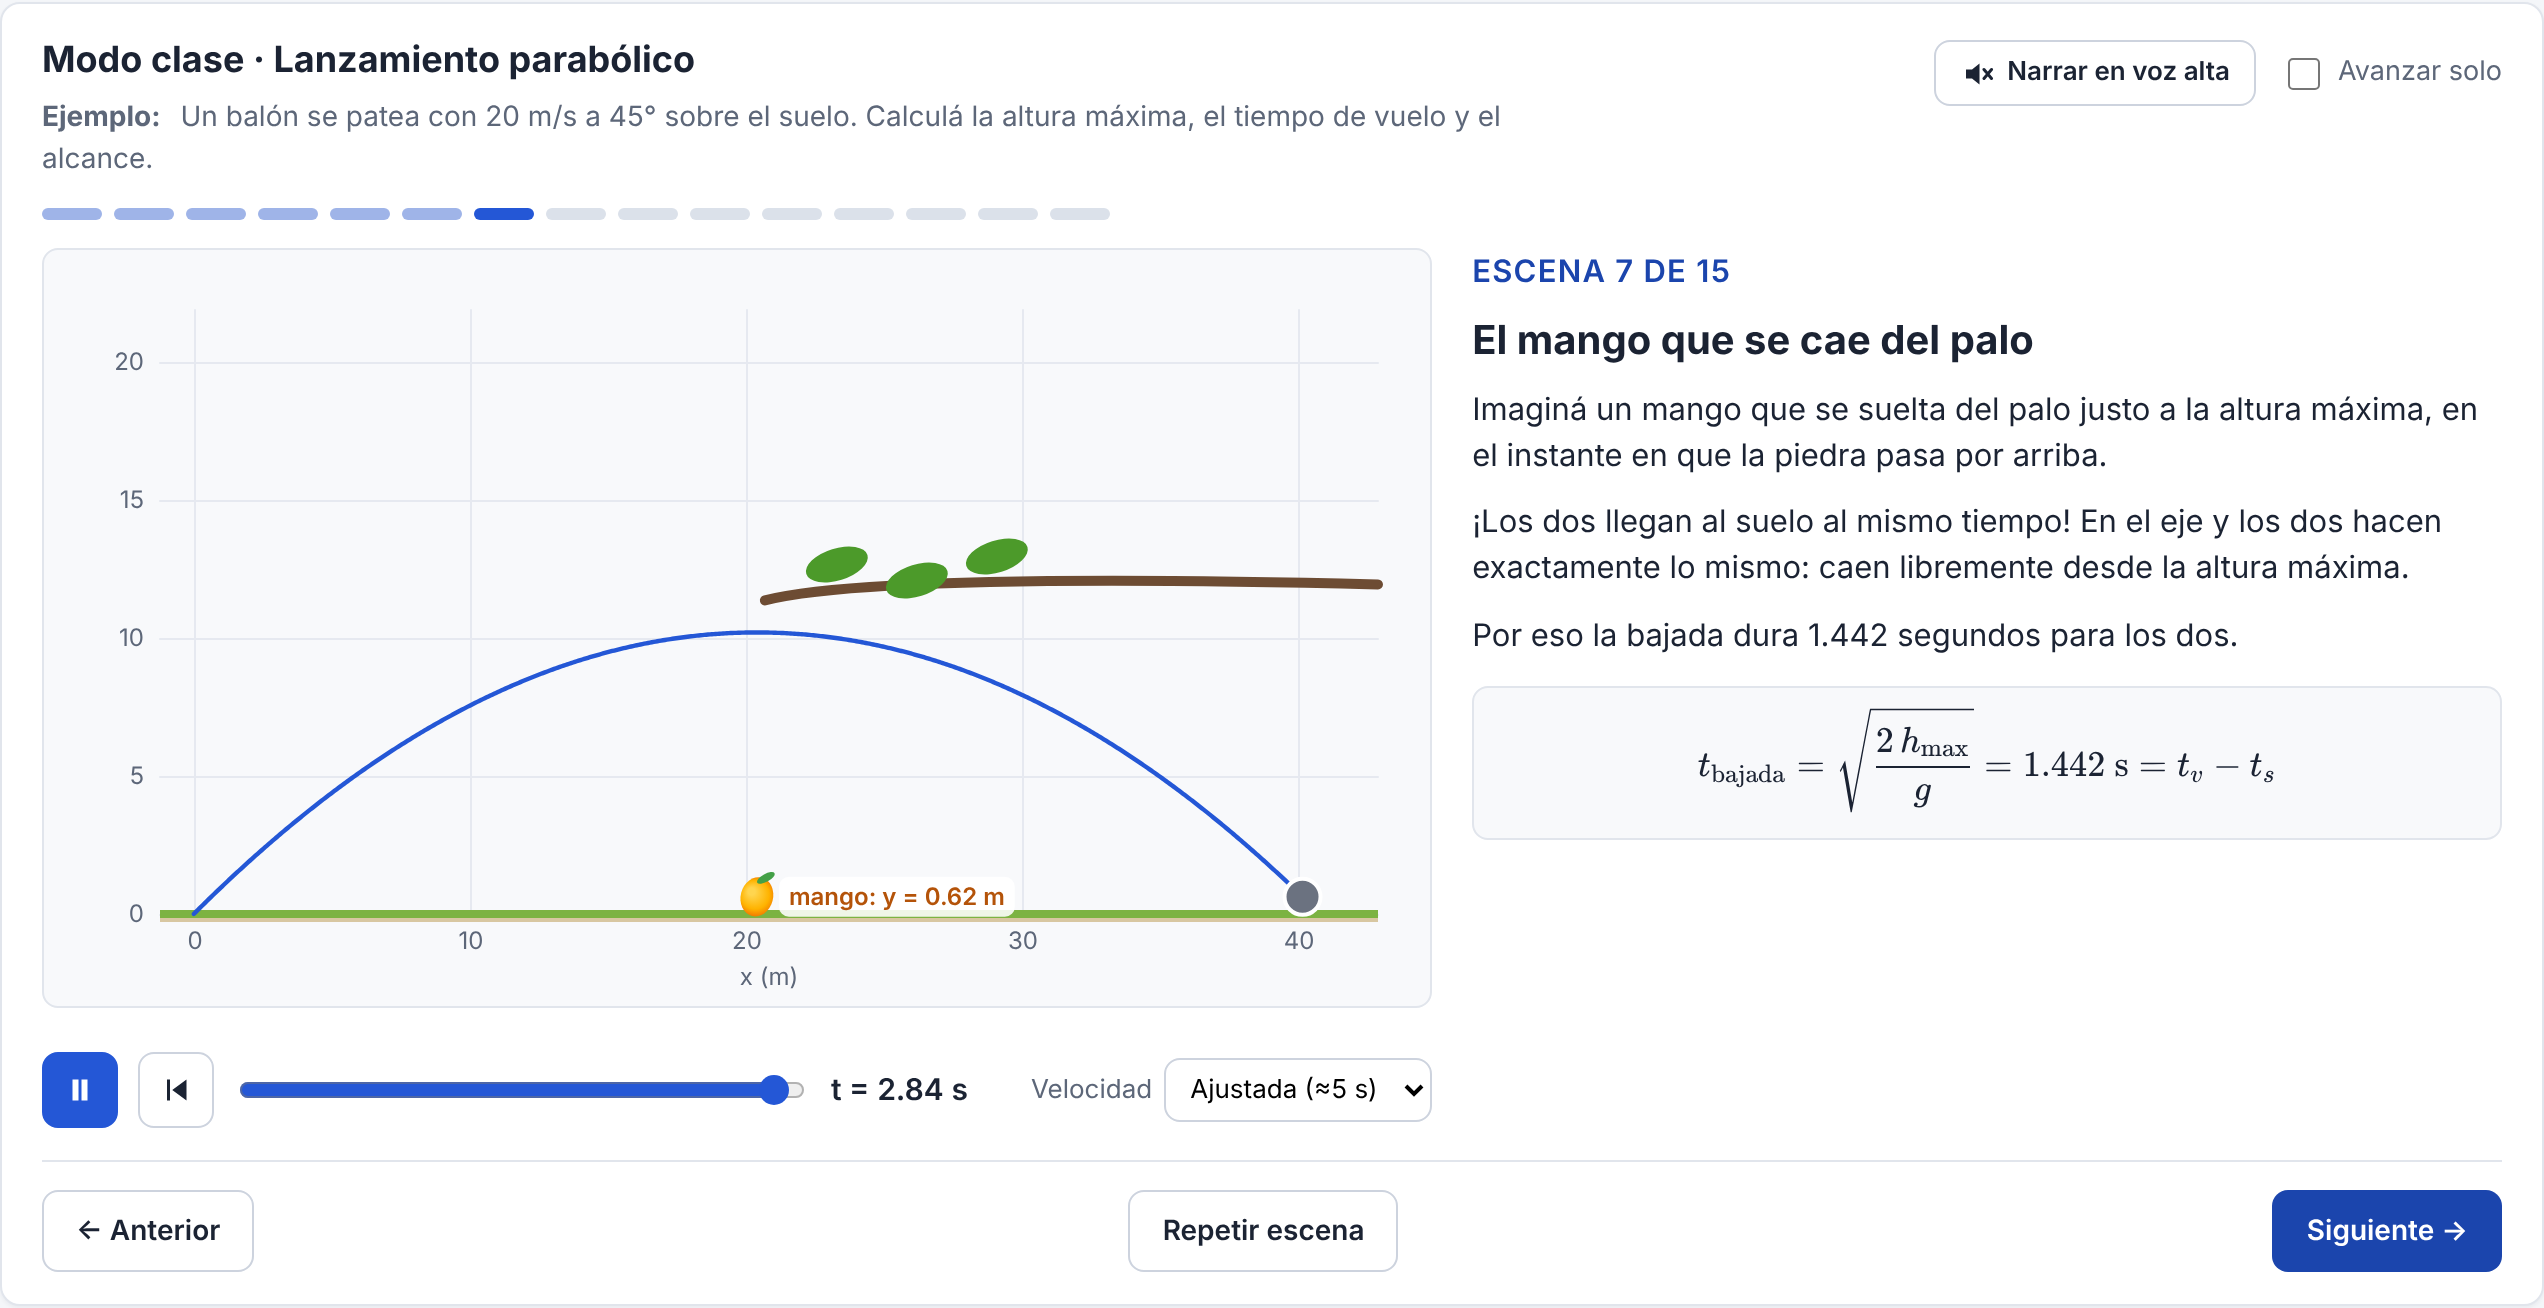
\includegraphics[width=0.49\linewidth]{img/clase_gemelo.png}\hfill
  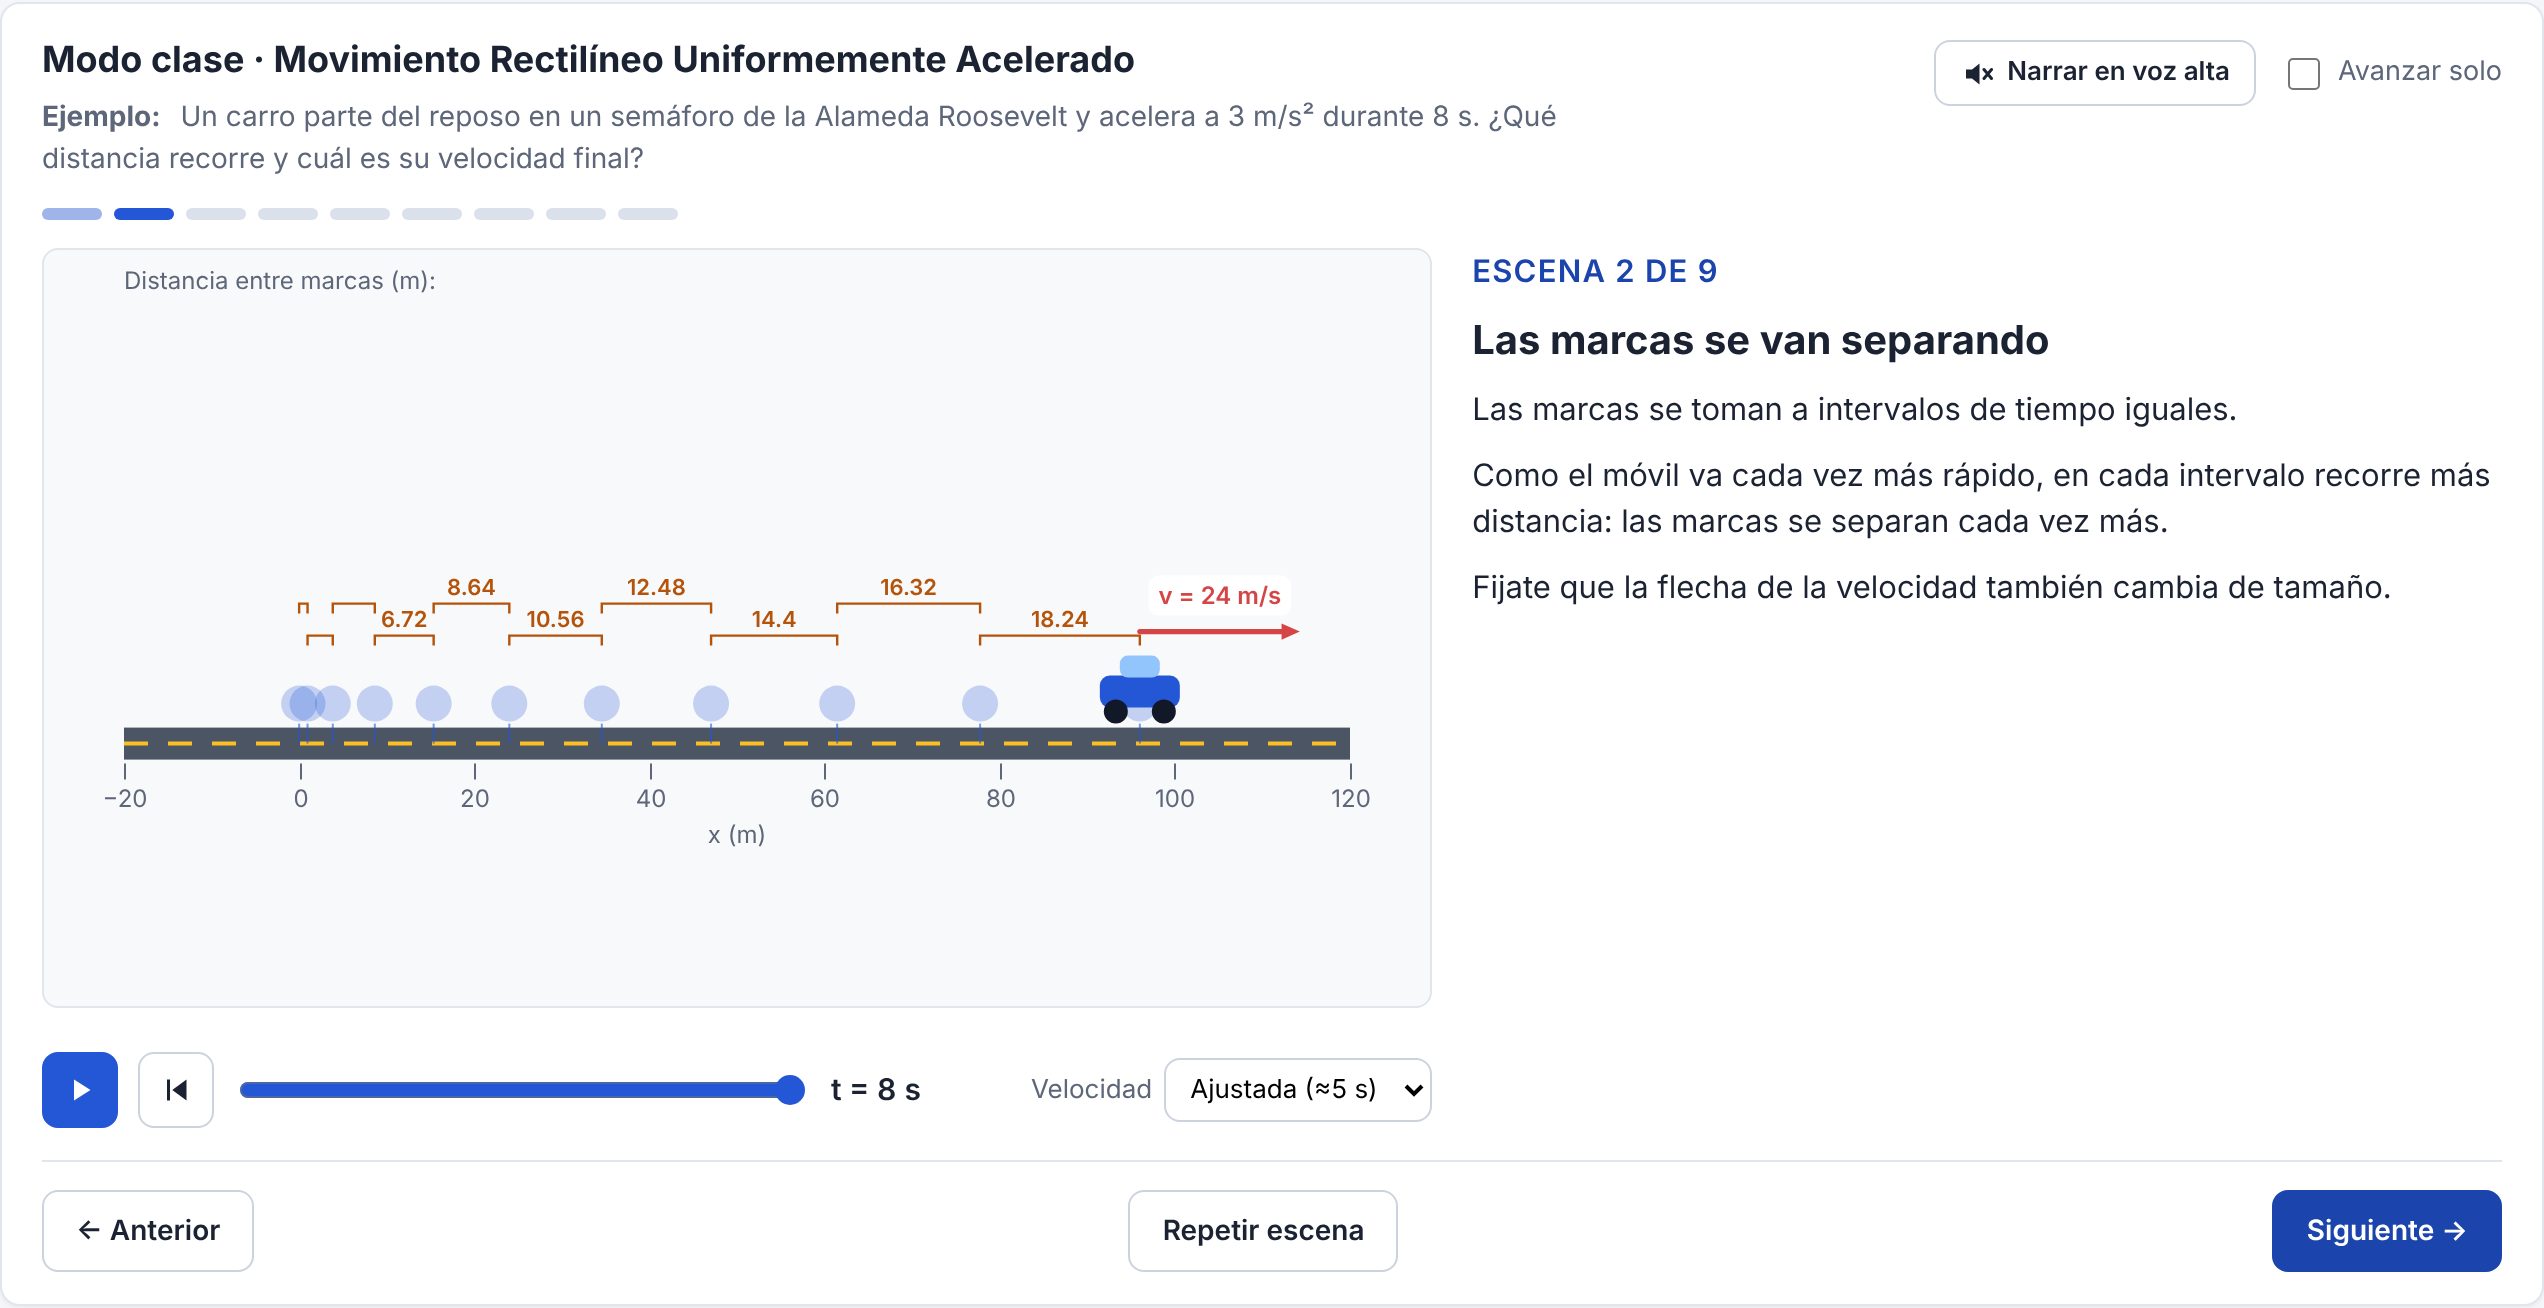
\includegraphics[width=0.49\linewidth]{img/clase_mrua.png}
  \caption{Izquierda: el mango que cae del palo llega al suelo junto con la piedra. Derecha: en el MRUA las marcas se separan cada vez más; la regla muestra la distancia entre marcas.}
\end{figure}

\subsection{Juego ``La hondilla''}

El jugador lanza piedras con una hondilla. Para apuntar, arrastra la piedra hacia atrás o usa los controles de ángulo y rapidez. Cada tiro se envía al motor, que calcula la trayectoria completa (60 puntos por segundo), detecta los choques cada $1/240$ s y decide qué objetivos caen. Una lata golpeada bota también las que tiene encima. La interfaz anima la respuesta.

\begin{table}[H]
\centering
\small
\begin{tabularx}{\linewidth}{@{}lX@{}}
\toprule
\textbf{Modo} & \textbf{Escenarios} \\
\midrule
Botá las latas & La cancha de la colonia · El parque de Juayúa · El muro de la escuela (muro de 7 m) · La azotea de la tienda (8 m) · El cerro de Apaneca (se tira desde 5 m de altura). \\
Bajá mangos & El palo de mango de la abuela · El palo de la cancha · El palo del vecino (detrás de un muro). El tronco detiene la piedra y la copa no. El mango golpeado cae en caída libre. \\
Hondillazos entre amigos & Hondillazos en el patio · Duelo entre cerros. Dos jugadores por turnos; gana quien bote primero las tres latas del otro. \\
\bottomrule
\end{tabularx}
\caption{Modos y escenarios del juego.}
\end{table}

Después de cada tiro, el motor devuelve:
\begin{itemize}
  \item una \textbf{frase salvadoreña}, como ``¡Chivo, cipote! Le diste.'', ``¡Púchica, casi!'' o ``¡Va para San Miguel ese tiro!'';
  \item un \textbf{veredicto}: si pasó por encima o por debajo y por cuánto, si se quedó corto o si chocó con algo;
  \item el \textbf{análisis}: componentes de la velocidad, punto más alto, ecuación de la trayectoria del tiro, altura a la que pasó por el objetivo, por qué chocó con el muro y, si cayó un mango, su caída libre;
  \item el \textbf{tiro perfecto}: la deducción de la ecuación \eqref{eq:perfecto} con los números del jugador, y otro ángulo si el suyo no funciona.
\end{itemize}
La opción \emph{Rayos X} muestra la sombra de la piedra en cada eje mientras vuela.

\begin{figure}[H]
  \centering
  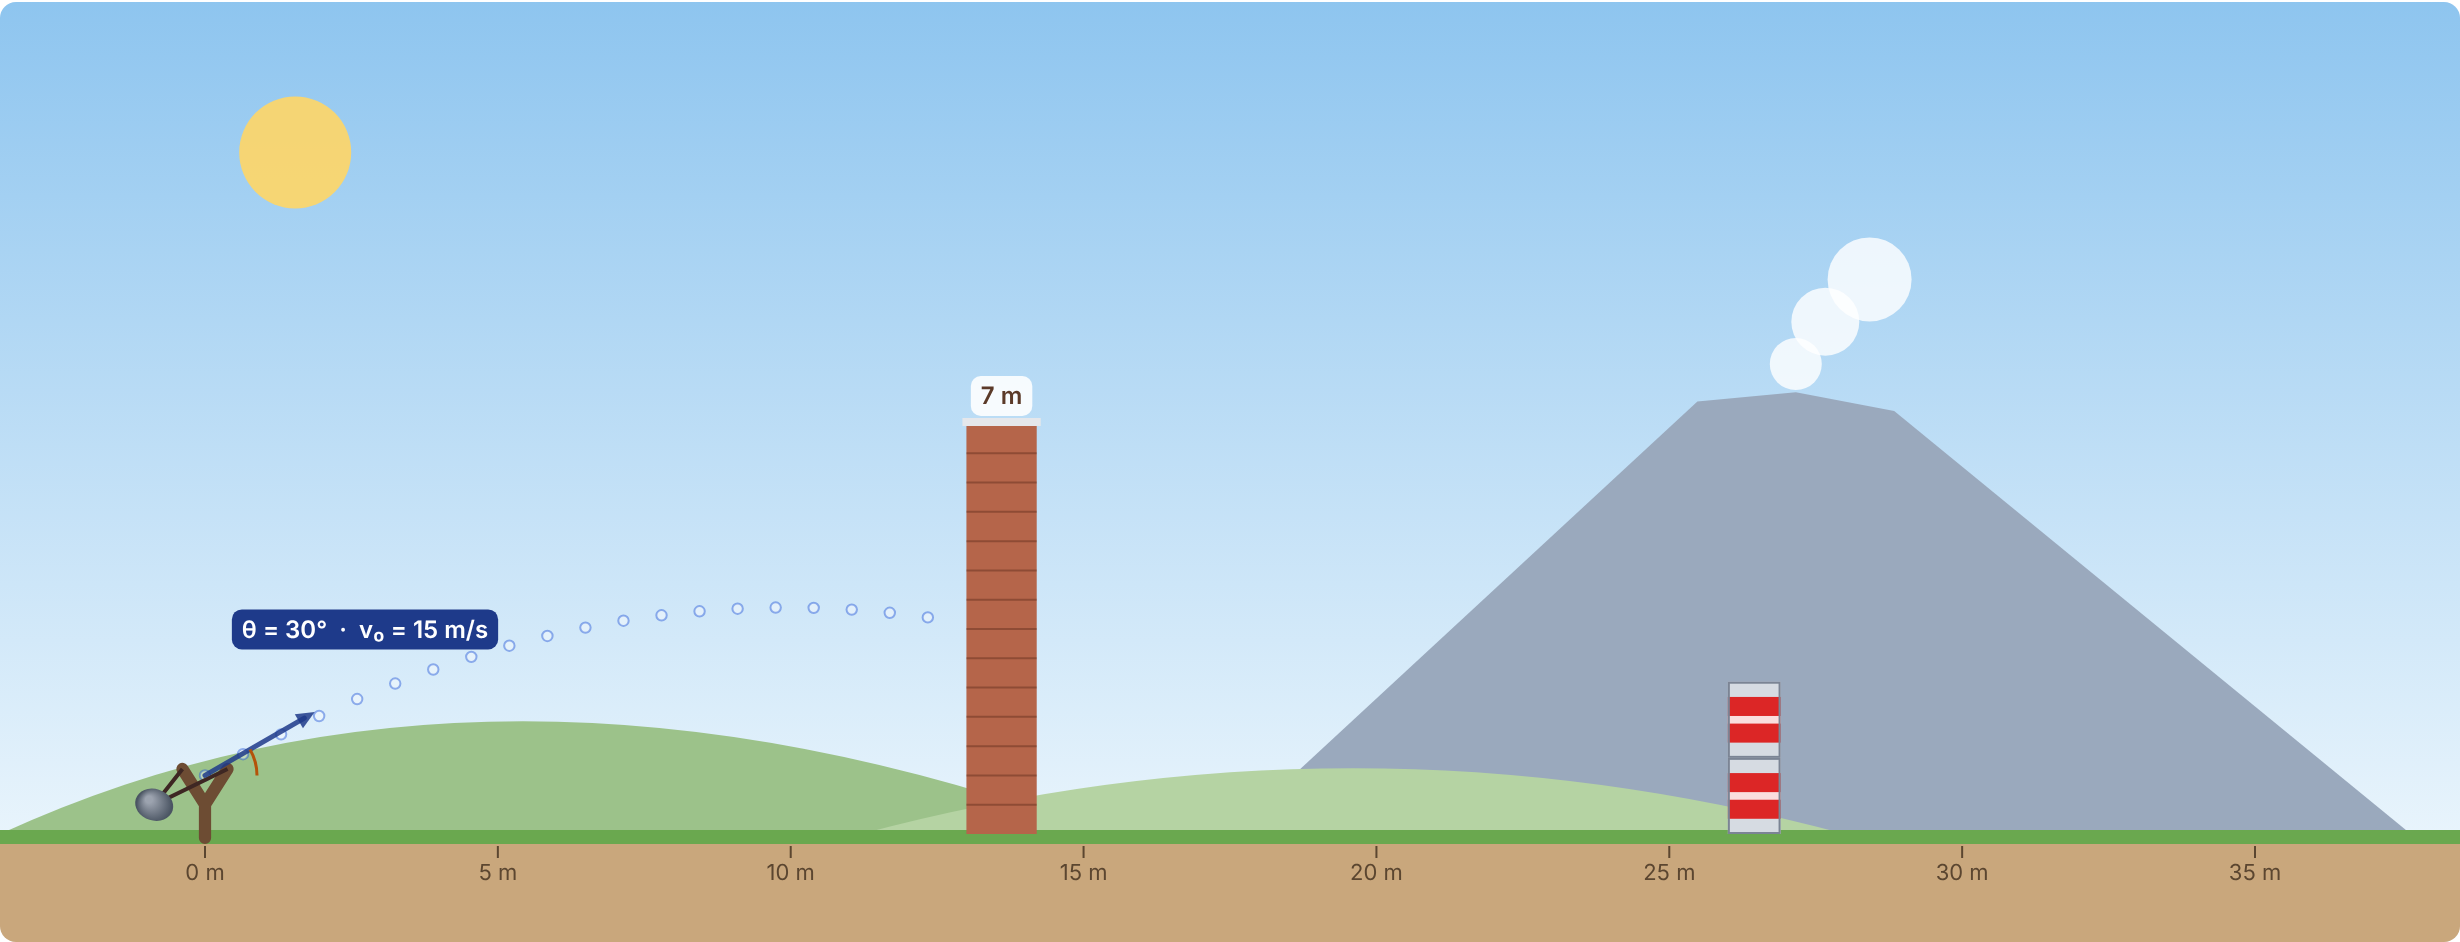
\includegraphics[width=0.49\linewidth]{img/juego_fallo.png}\hfill
  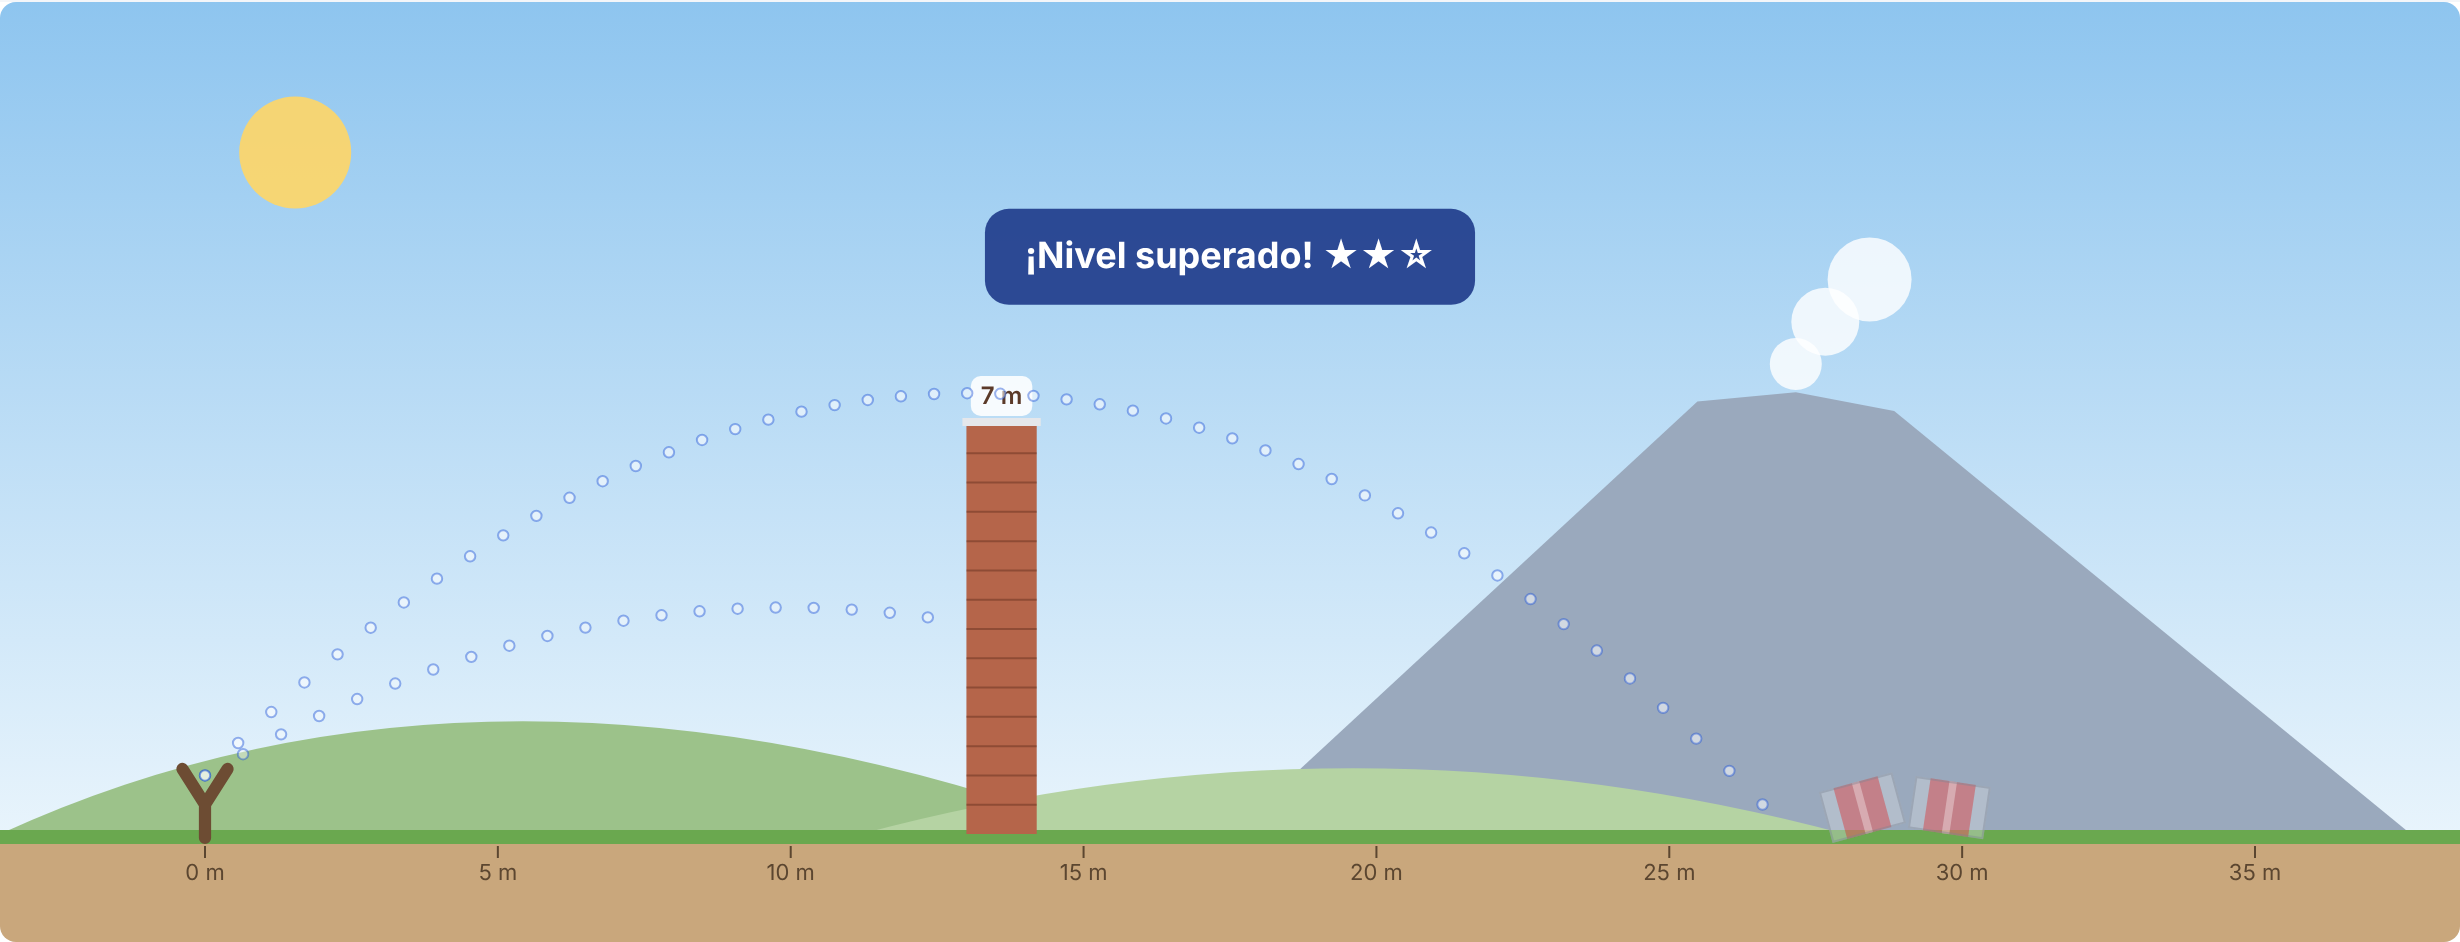
\includegraphics[width=0.49\linewidth]{img/juego_acierto.png}
  \caption{``El muro de la escuela''. Izquierda: con $\theta = 30^\circ$ y $v_0 = 15$ m/s la piedra choca con el muro. Derecha: con el tiro perfecto ($45^\circ$, 16.00 m/s) pasa el muro y bota las latas.}
\end{figure}

\begin{figure}[H]
  \centering
  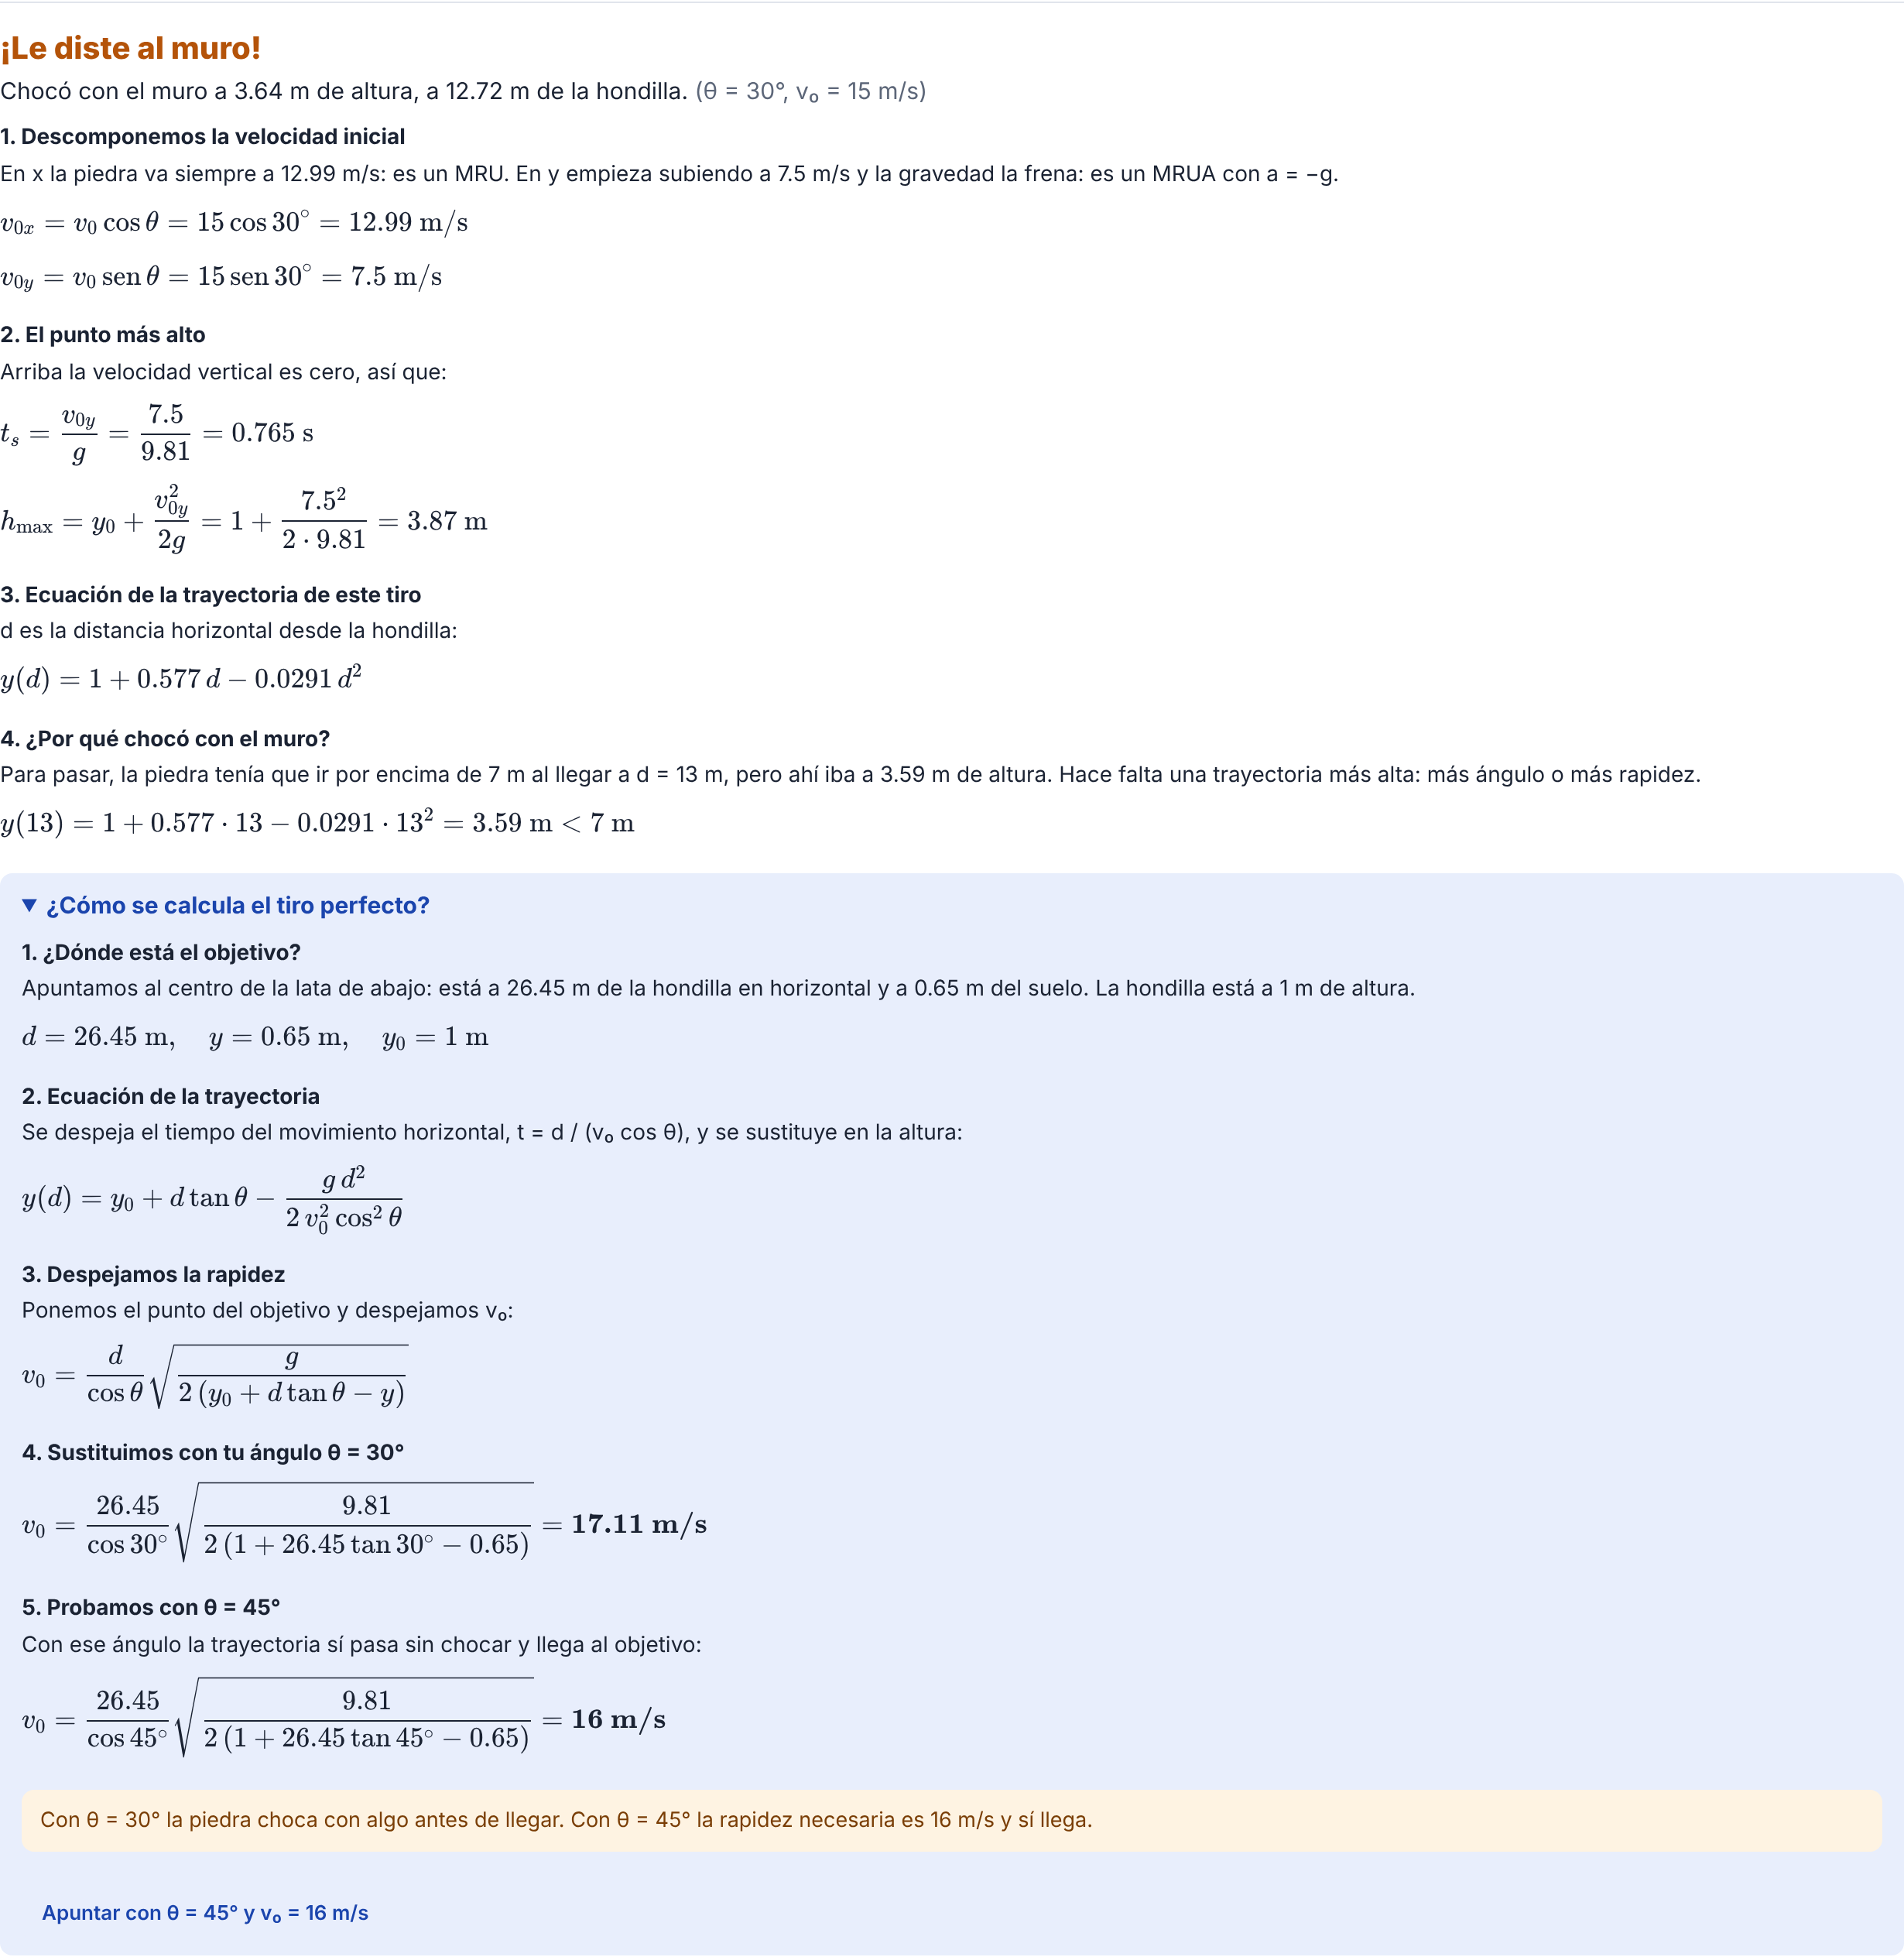
\includegraphics[width=0.78\linewidth]{img/juego_analisis.png}
  \caption{Análisis del tiro fallido y deducción del tiro perfecto.}
\end{figure}

\begin{figure}[H]
  \centering
  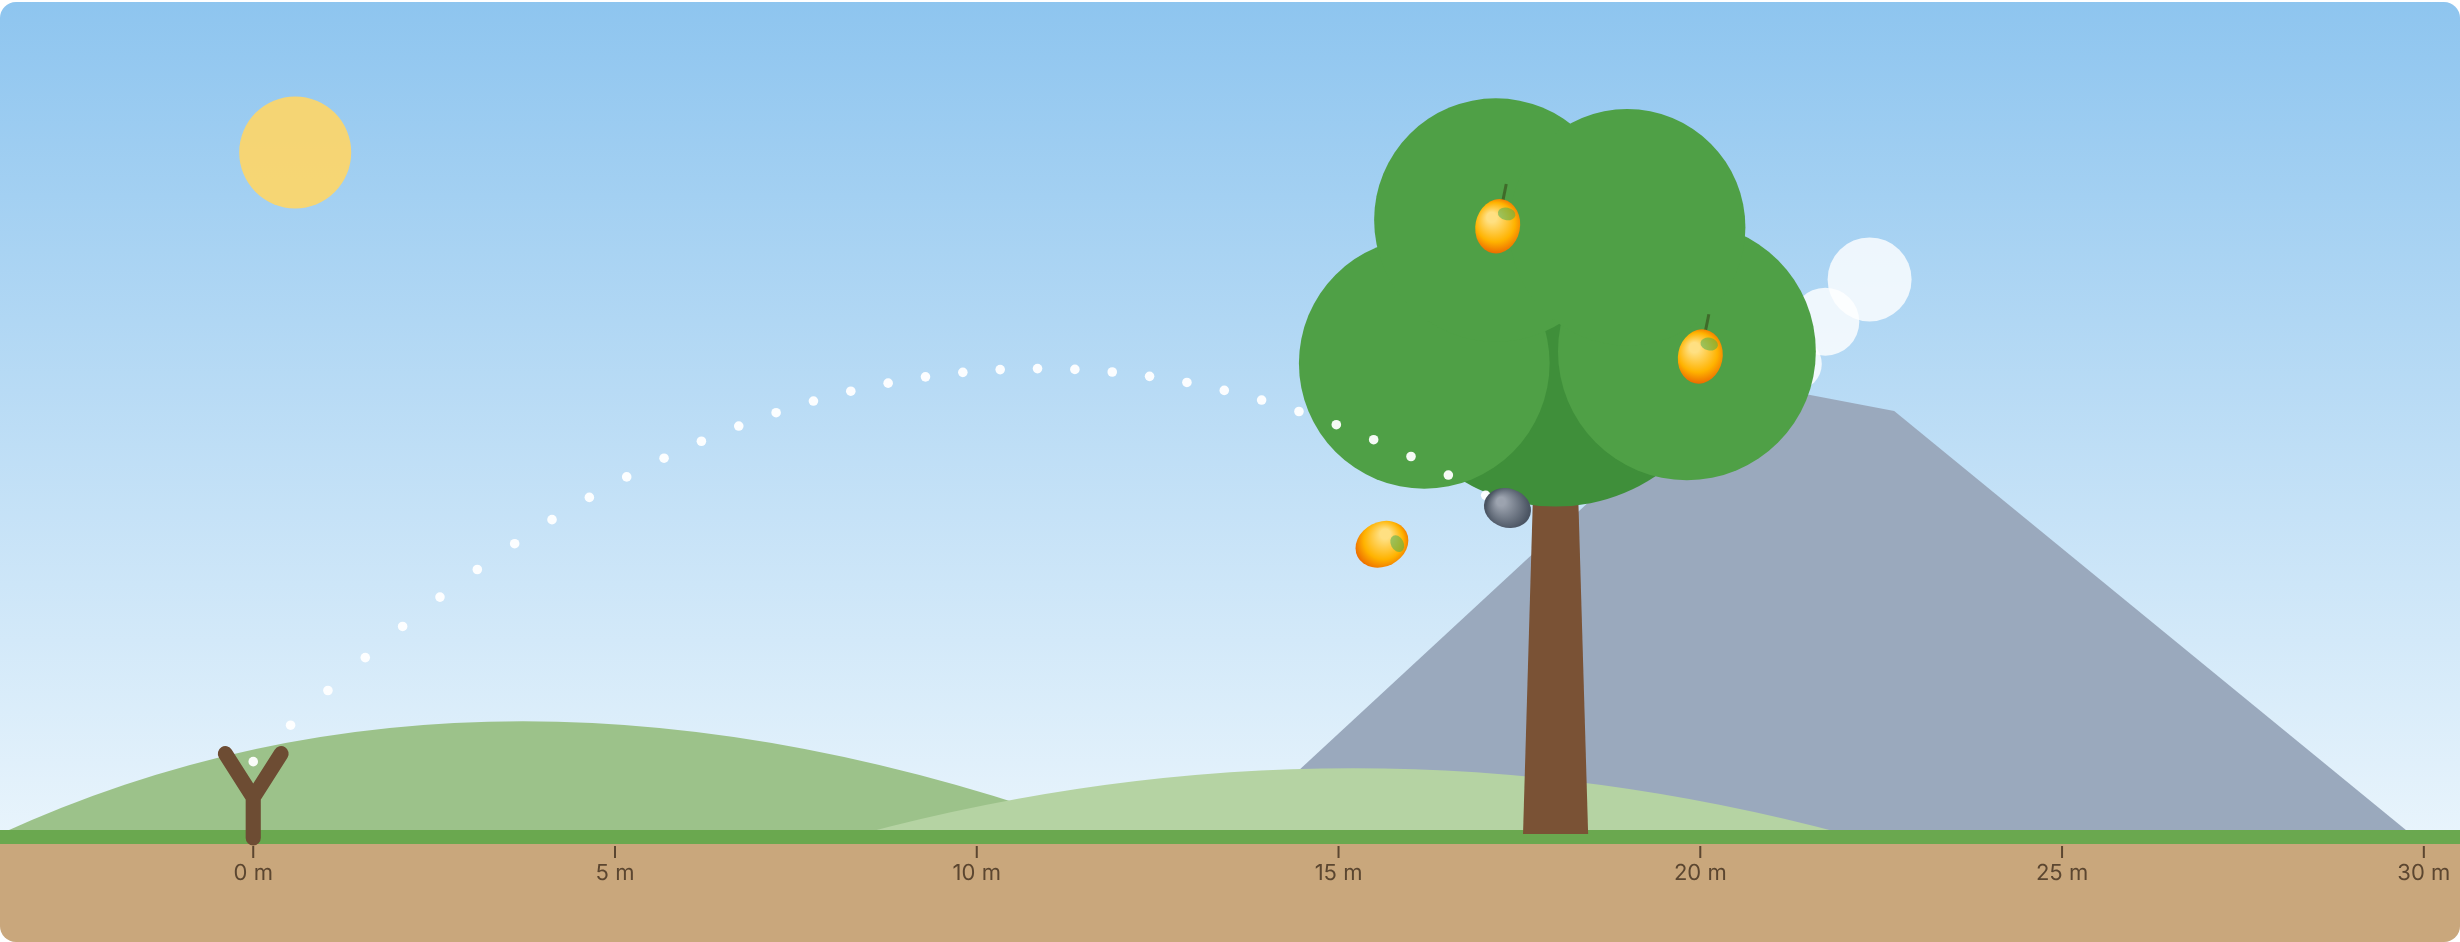
\includegraphics[width=0.49\linewidth]{img/juego_mangos.png}\hfill
  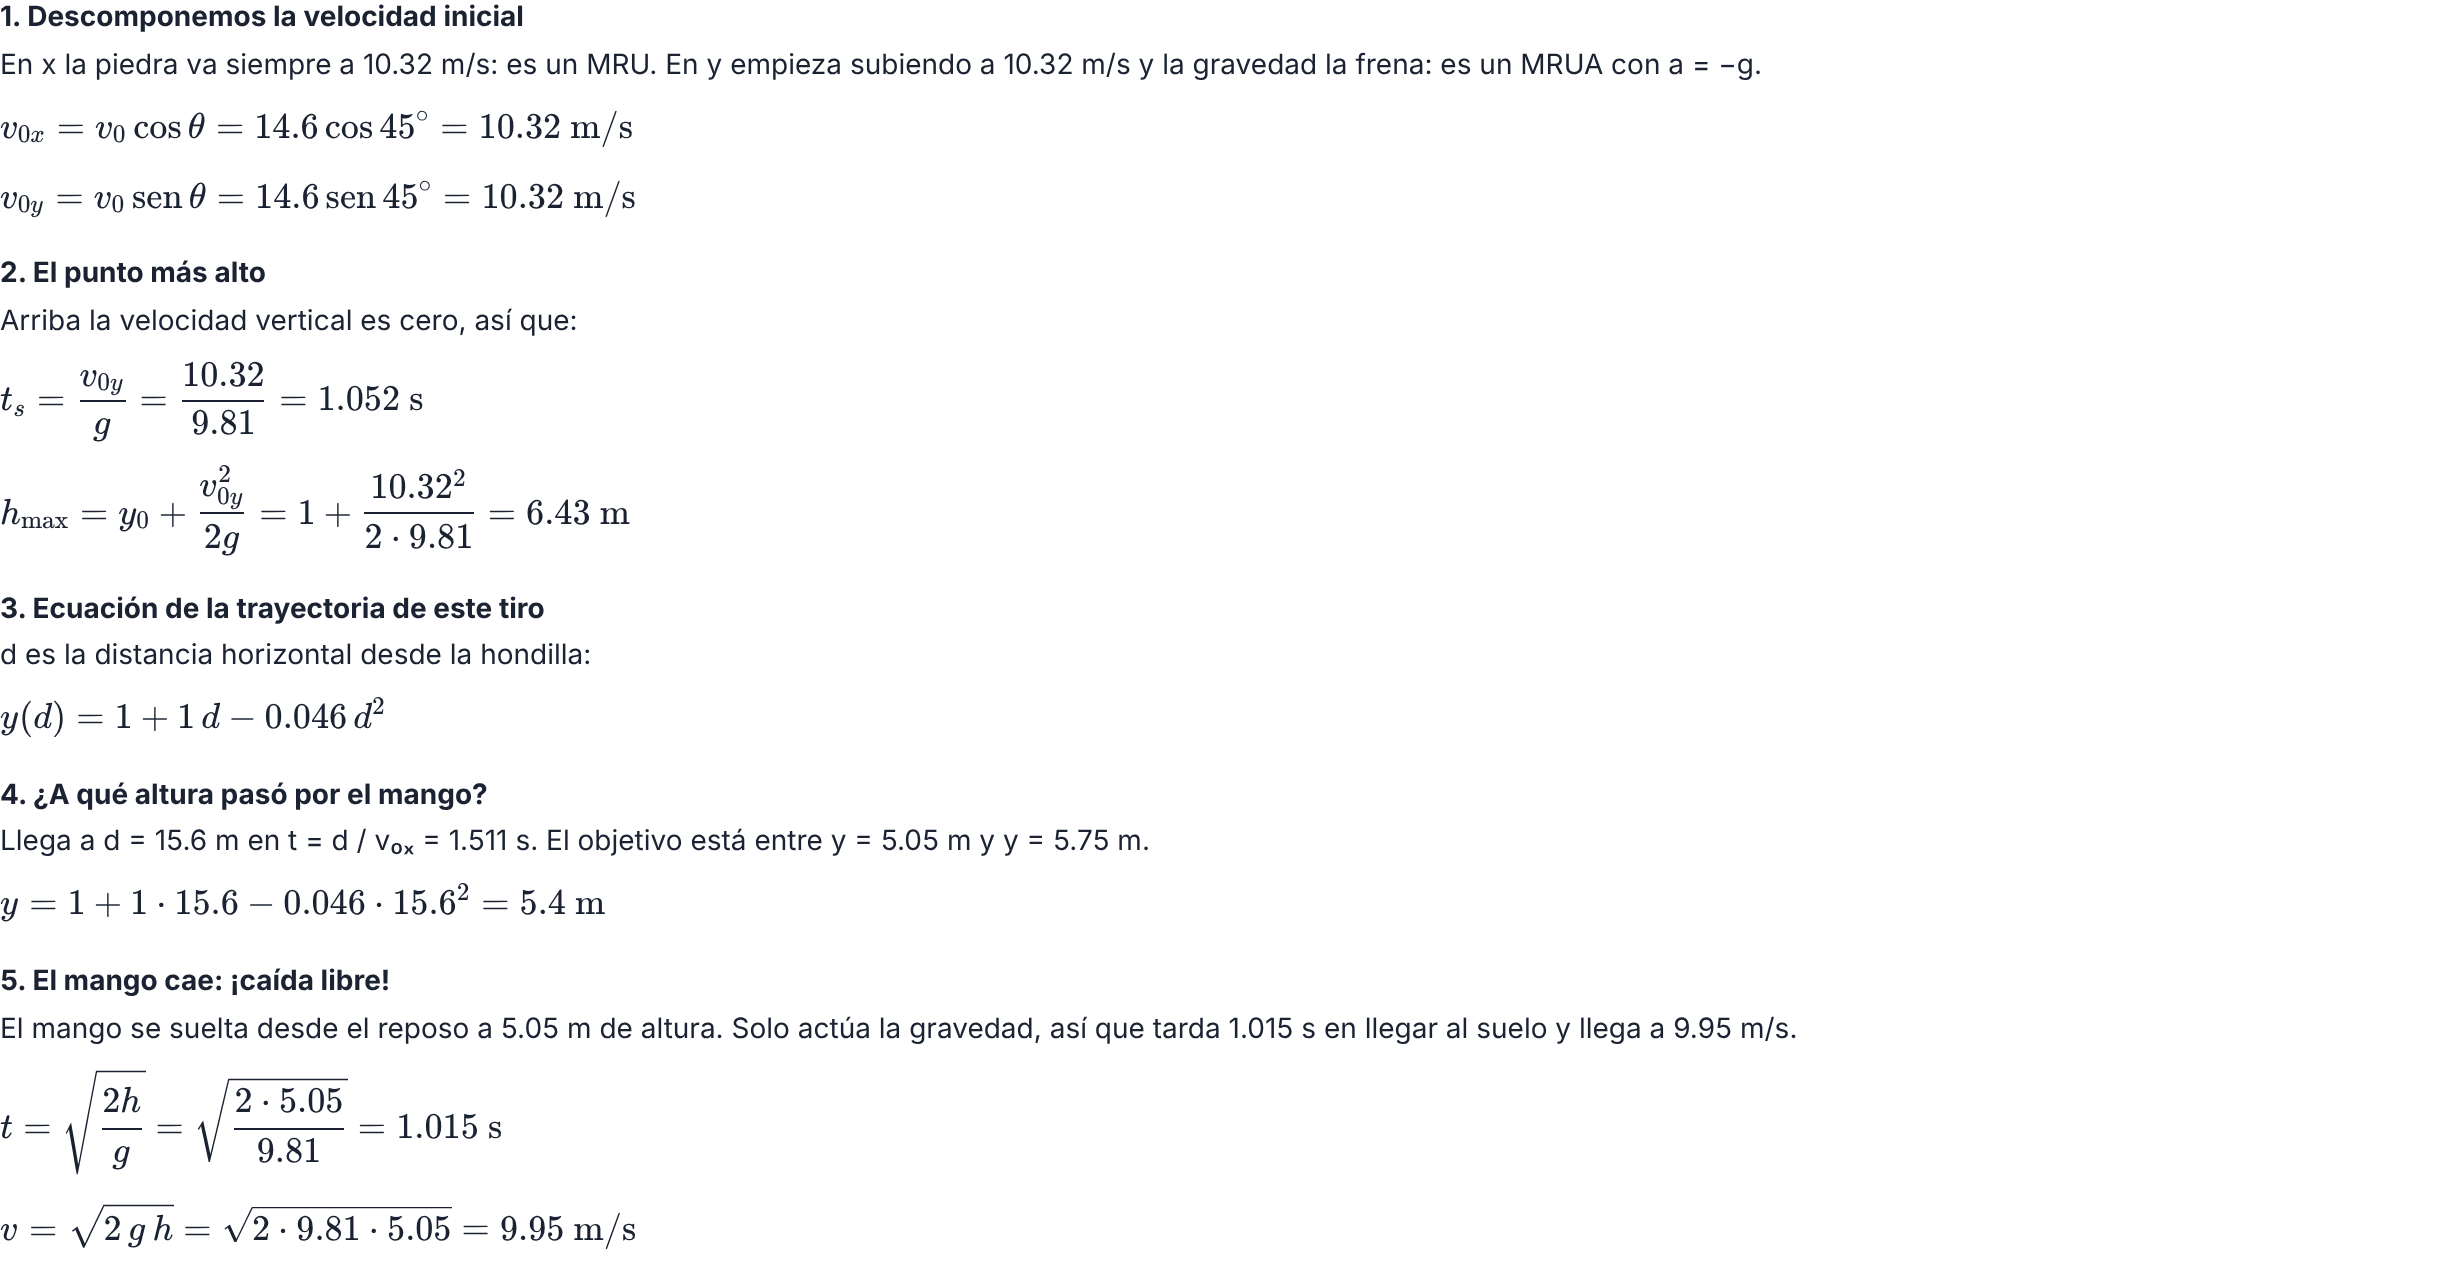
\includegraphics[width=0.49\linewidth]{img/juego_mango_analisis.png}
  \caption{``Bajá mangos'': la piedra golpea un mango, que cae en caída libre. El análisis calcula su tiempo de caída y su rapidez al llegar al suelo.}
\end{figure}

\begin{figure}[H]
  \centering
  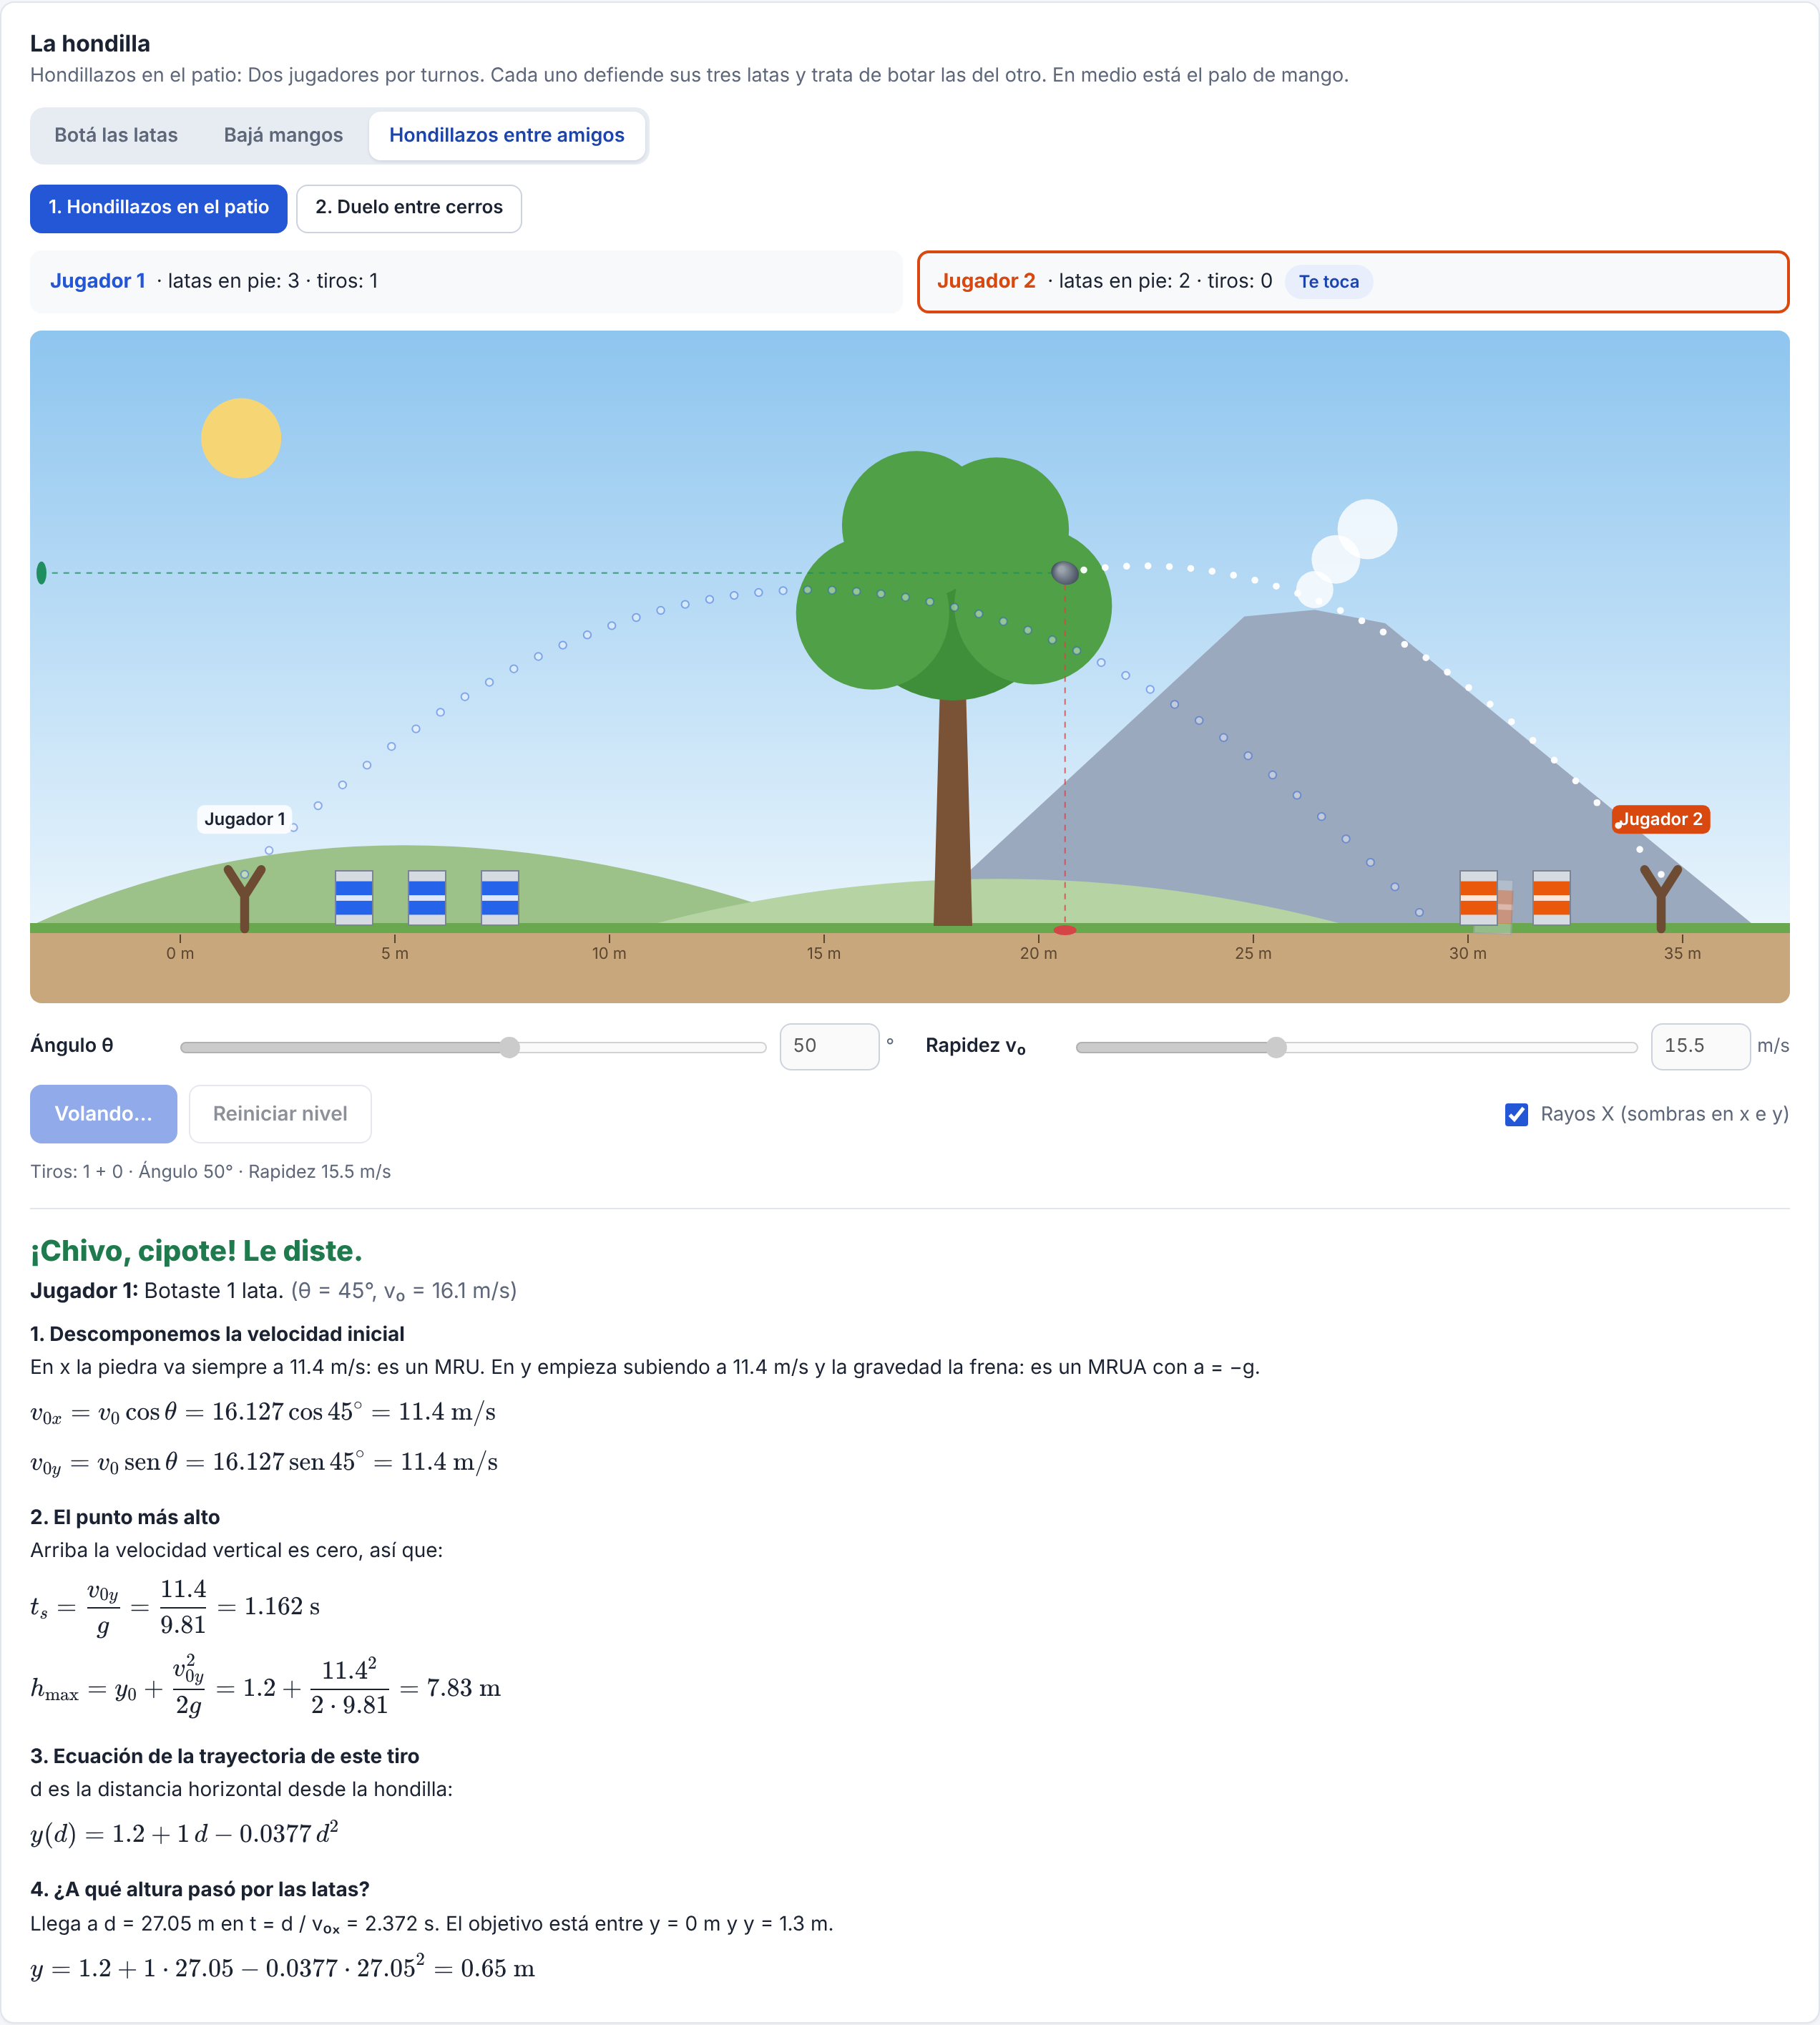
\includegraphics[width=0.85\linewidth]{img/juego_duelo.png}
  \caption{``Hondillazos entre amigos'' con la opción Rayos X activa: marcador, turno y tiro del Jugador 2.}
\end{figure}

% ================================================================ 11
\section{Interfaz y animación}

\begin{itemize}
  \item \textbf{Animación fiel al cálculo}: un reloj con \texttt{requestAnimationFrame} avanza el tiempo, y la posición se obtiene interpolando las muestras del motor. Lo que se ve es lo que se calculó.
  \item \textbf{Capas didácticas}: cada escena del Modo clase enciende capas distintas: marcas, regla, vectores, trayectoria, sombras, componentes, punto alto y mango gemelo.
  \item \textbf{Notación matemática real}: el motor escribe las fórmulas en \LaTeX{} y KaTeX las muestra en la página.
  \item \textbf{Ambiente salvadoreño}: un volcán humeando, cerros, palos de mango, el tapial de la escuela, la tienda de la esquina y hondillas de madera.
  \item \textbf{Accesibilidad}: etiquetas visibles en todos los campos y navegación con teclado (pestañas con flechas y Modo clase con flechas). Si el sistema tiene activada la opción de reducir el movimiento, las animaciones no arrancan solas.
  \item \textbf{Diseño adaptable}: en el teléfono todo se apila en una columna, sin desplazamiento horizontal (figura~\ref{fig:movil}).
\end{itemize}

\begin{figure}[H]
  \centering
  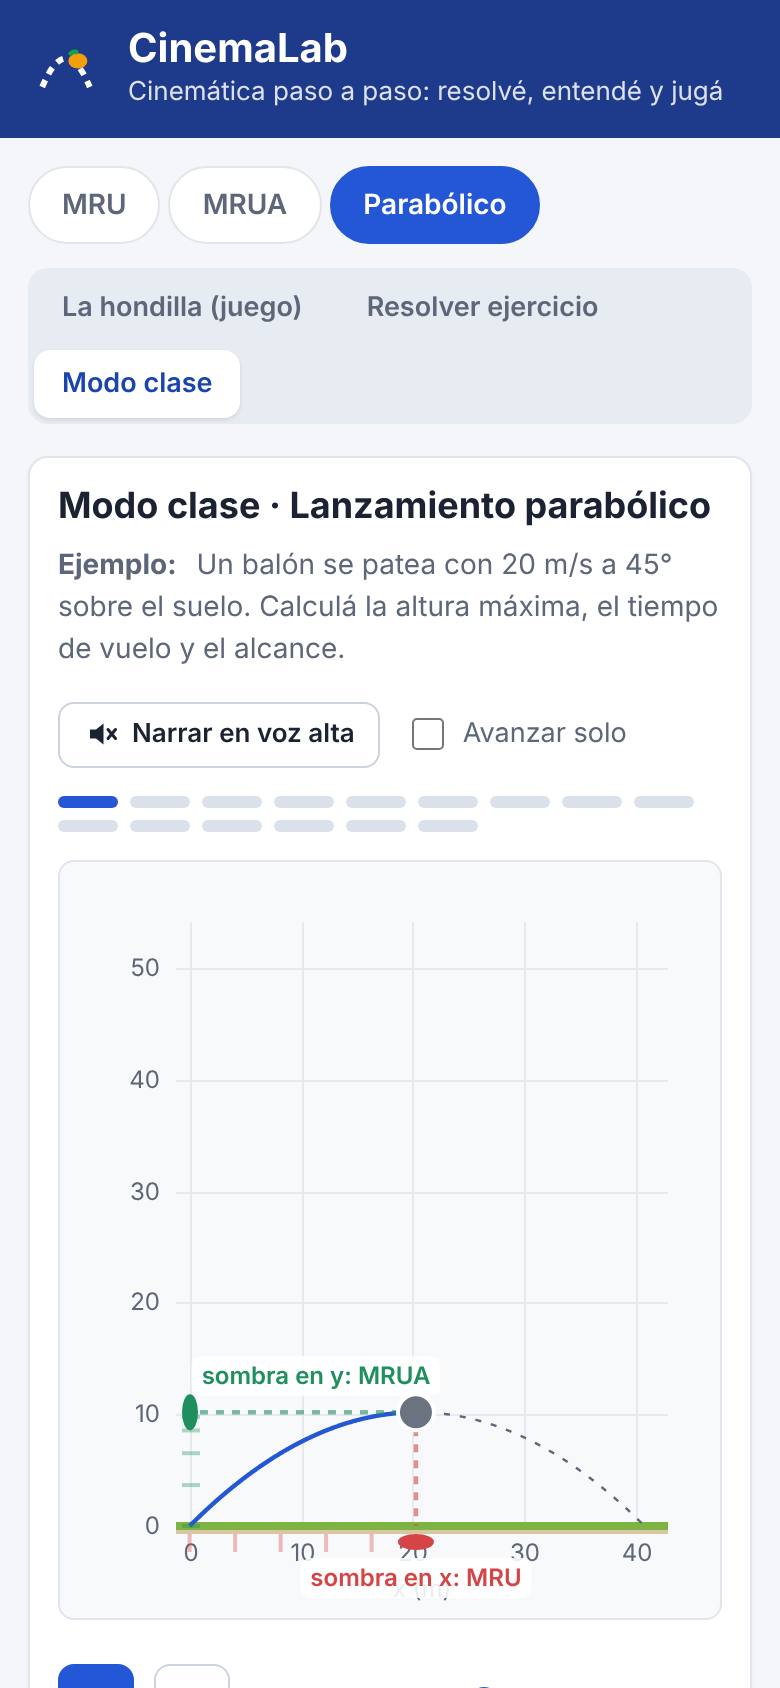
\includegraphics[width=0.28\linewidth]{img/movil.png}
  \caption{Modo clase en un teléfono (390 px de ancho).}
  \label{fig:movil}
\end{figure}

% ================================================================ 12
\section{Distribución del trabajo}

\begin{table}[H]
\centering
\small
\begin{tabularx}{\linewidth}{@{}lX@{}}
\toprule
\textbf{Integrante} & \textbf{Responsabilidades} \\
\midrule
Dennis Ariel Avila Fuentes & \pend{Por ejemplo: arquitectura, motor en Rust y API en Node.js} \\
\pend{Integrante 2} & \pend{Por ejemplo: interfaz en React, Modo clase y juego} \\
\pend{Integrante 3} & \pend{Por ejemplo: pruebas, ejercicios de ejemplo e informe} \\
\bottomrule
\end{tabularx}
\caption{Distribución del trabajo.}
\end{table}

% ================================================================ 13
\section{Pruebas y resultados}
\label{sec:pruebas}

\subsection{Pruebas del motor (Rust)}

Con \texttt{cargo test} se ejecutan 14 pruebas: 2 unitarias y 12 de validación. Cada ejercicio de ejemplo se comparó con un cálculo independiente hecho con las fórmulas cerradas.

\begin{table}[H]
\centering
\small
\begin{tabular}{@{}llcrrc@{}}
\toprule
\textbf{Tema} & \textbf{Ejercicio} & \textbf{Variable} & \textbf{Esperado} & \textbf{Obtenido} & \textbf{Pasos} \\
\midrule
MRU & El microbús de la ruta & $\Delta x$ (m) & 600.0000 & 600.0000 & 1 \\
MRU & Ciclista en la Ruta Militar & $v$ (m/s) & 8.0000 & 8.0000 & 1 \\
MRU & Caminando al mercado & $t$ (s) & 360.0000 & 360.0000 & 1 \\
MRUA & Arranque en el semáforo & $\Delta x$ (m) & 96.0000 & 96.0000 & 2 \\
MRUA & Arranque en el semáforo & $v$ (m/s) & 24.0000 & 24.0000 & 2 \\
MRUA & Frenado en la carretera & $a$ (m/s$^2$) & $-$6.2500 & $-$6.2500 & 2 \\
MRUA & Frenado en la carretera & $t$ (s) & 4.0000 & 4.0000 & 2 \\
MRUA & Moto en la Panamericana & $\Delta x$ (m) & 200.0000 & 200.0000 & 2 \\
MRUA & Moto en la Panamericana & $t$ (s) & 10.0000 & 10.0000 & 2 \\
Parabólico & Penal en la cancha & $h_{\max}$ (m) & 10.1937 & 10.1937 & 5 \\
Parabólico & Penal en la cancha & $t_v$ (s) & 2.8832 & 2.8832 & 5 \\
Parabólico & Penal en la cancha & $R$ (m) & 40.7747 & 40.7747 & 5 \\
Parabólico & Cohete de pólvora & $v_0$ (m/s) & 30.1033 & 30.1033 & 1 \\
Parabólico & Piedra desde el mirador & $t_v$ (s) & 3.3582 & 3.3582 & 4 \\
Parabólico & Piedra desde el mirador & $R$ (m) & 40.2292 & 40.2292 & 4 \\
\bottomrule
\end{tabular}
\caption{Validación del motor con los 9 ejercicios de ejemplo (15 resultados, diferencia relativa menor que $10^{-9}$).}
\end{table}

Las demás pruebas del motor comprueban lo siguiente:
\begin{itemize}
  \item datos insuficientes, datos inconsistentes, tiempos negativos, alcance imposible y valores fuera de rango;
  \item que al calcular el ángulo desde el alcance aparezcan las dos soluciones;
  \item que la simulación termine donde dice la solución ($x(T) = \Delta x$ o $R$, $y(T) = 0$ y $y(t_s) = h_{\max}$);
  \item que las lecciones se generen con los datos de ejemplo y con los del usuario;
  \item que el mango caiga con $t = \sqrt{2h/g}$ y que un tiro de $30^\circ$ a 15 m/s choque con el muro;
  \item que \textbf{todos los escenarios del juego se puedan ganar} siguiendo el tiro perfecto, incluyendo los dos jugadores de cada duelo (tabla~\ref{tab:juego}).
\end{itemize}

\begin{table}[H]
\centering
\footnotesize
\begin{tabular}{@{}lllcccc@{}}
\toprule
\textbf{Modo} & \textbf{Escenario} & \textbf{Jugador} & \textbf{Objetivos} & \textbf{1.\textsuperscript{er} tiro ($\theta$ / $v_0$)} & \textbf{Tiros} & \textbf{Ganado} \\
\midrule
Botá las latas & La cancha de la colonia & Vos & 2 & 45$^\circ$ / 13.33 & 1 & Sí \\
Botá las latas & El parque de Juayúa & Vos & 3 & 45$^\circ$ / 17.47 & 1 & Sí \\
Botá las latas & El muro de la escuela & Vos & 2 & 45$^\circ$ / 16.00 & 1 & Sí \\
Botá las latas & La azotea de la tienda & Vos & 2 & 45$^\circ$ / 19.11 & 1 & Sí \\
Botá las latas & El cerro de Apaneca & Vos & 3 & 46$^\circ$ / 18.18 & 1 & Sí \\
Bajá mangos & El palo de mango de la abuela & Vos & 3 & 45$^\circ$ / 14.60 & 3 & Sí \\
Bajá mangos & El palo de la cancha & Vos & 4 & 45$^\circ$ / 18.02 & 4 & Sí \\
Bajá mangos & El palo del vecino & Vos & 3 & 45$^\circ$ / 17.62 & 3 & Sí \\
Hondillazos & Hondillazos en el patio & Jugador 1 & 3 & 45$^\circ$ / 16.13 & 3 & Sí \\
Hondillazos & Hondillazos en el patio & Jugador 2 & 3 & 45$^\circ$ / 16.13 & 3 & Sí \\
Hondillazos & Duelo entre cerros & Jugador 1 & 3 & 45$^\circ$ / 16.83 & 3 & Sí \\
Hondillazos & Duelo entre cerros & Jugador 2 & 3 & 45$^\circ$ / 19.70 & 3 & Sí \\
\bottomrule
\end{tabular}
\caption{Cada escenario jugado con el tiro perfecto que sugiere el motor.}
\label{tab:juego}
\end{table}

En ``El cerro de Apaneca'', el tiro a $45^\circ$ chocaba con el muro de 10 m. El motor lo detectó y sugirió $46^\circ$ con 18.18 m/s, que sí pasa.

\subsection{Pruebas de la API (Node.js)}

Con Vitest y \texttt{app.inject()} de Fastify, sin abrir puertos, se ejecutan 10 pruebas. Verifican la salud y la versión del motor, la lista de modelos y la resolución de un MRUA con su simulación. También comprueban el rechazo de datos mal formados (400), los errores de rango del motor, la generación de una lección, un tiro que choca con el muro, que el tiro perfecto sí acierte, un escenario inexistente (422) y un ángulo fuera de rango (400).

\subsection{Pruebas de la interfaz y de punta a punta}

Con Vitest se prueban el formato de números (coma decimal y signo menos) y la interpolación de muestras. Con Playwright se controló Google Chrome para recorrer la aplicación completa:
\begin{itemize}
  \item resolver ejemplos y datos escritos a mano, con validación y avisos;
  \item avanzar por las escenas del Modo clase de los tres temas;
  \item ganar un nivel de ``Bajá mangos'' (3 tiros) y un duelo completo (5 tiros alternando jugadores);
  \item apuntar arrastrando con el ratón;
  \item comprobar que en una pantalla de teléfono de 390 px no hay desplazamiento horizontal.
\end{itemize}

\subsection{Rendimiento}

\begin{table}[H]
\centering
\small
\begin{tabular}{@{}lcc@{}}
\toprule
\textbf{Operación} & \textbf{Tiempo medio por petición} & \textbf{Tamaño de la respuesta} \\
\midrule
\texttt{POST /api/resolver} (parabólico, con simulación) & 3.0 ms & 55 KB \\
\texttt{POST /api/leccion} (parabólico, 15 escenas) & 3.1 ms & 64 KB \\
\texttt{POST /api/juego/tiro} & 1.2 ms & 5 KB \\
\texttt{POST /api/juego/sugerencia} & 1.0 ms & 1.4 KB \\
\bottomrule
\end{tabular}
\caption{Tiempos de la API, con 200 peticiones seguidas en la computadora de pruebas.}
\end{table}

En Chrome, la animación del resolvedor, la del Modo clase y la del juego corren a \textbf{60 cuadros por segundo}, sin cuadros de más de 16.8 ms.

\subsection{Resumen}

\begin{table}[H]
\centering
\small
\begin{tabular}{@{}llc@{}}
\toprule
\textbf{Capa} & \textbf{Herramienta} & \textbf{Resultado} \\
\midrule
Motor (Rust) & cargo test & 14 de 14 \\
API (Node.js) & Vitest & 10 de 10 \\
Interfaz (React) & Vitest & 4 de 4 \\
Punta a punta & Playwright + Chrome & todos los flujos sin errores \\
Calidad de código & clippy, tsc estricto & sin advertencias \\
\bottomrule
\end{tabular}
\caption{Resumen de las pruebas.}
\end{table}

% ================================================================ 14
\section{Control de versiones y despliegue}

\subsection{Repositorio}

El código se maneja con Git y GitHub, en \pend{https://github.com/usuario/cinemalab}. La rama \texttt{main} tiene la versión estable, y el trabajo se hace en ramas por capa (\texttt{motor}, \texttt{api}, \texttt{web}, \texttt{informe}) que se integran con \emph{pull requests}. Antes de integrar, se ejecuta \texttt{pnpm test}.

\subsection{Ejecución local}

Se necesitan Rust (con rustup), Node.js 20 o más reciente, y pnpm.

\begin{lstlisting}[language=bash,caption={Comandos del proyecto.}]
pnpm install      # dependencias
pnpm dev          # compila el motor y levanta API (puerto 3000) y web (5173)
pnpm test         # cargo test + pruebas de la API y de la web
pnpm build        # compila motor, web y API para producción
pnpm start        # todo en http://localhost:3000
\end{lstlisting}

\subsection{Publicación}

Como la API corre en Node.js con un módulo nativo, la aplicación necesita un servidor. No puede publicarse en un hosting estático. El repositorio incluye un \texttt{Dockerfile} de dos etapas: la primera compila Rust, la web y la API, y la segunda produce una imagen solo con Node.js. También incluye un \texttt{render.yaml} para publicar en Render con su plan gratuito. Render compila la imagen y deja la aplicación en una dirección pública: \pend{https://cinemalab.onrender.com}. La ruta \texttt{/api/salud} sirve como verificación de estado.

% ================================================================ 15
\section{Limitaciones y aspectos pendientes}

\begin{itemize}
  \item \textbf{Sin resistencia del aire}: los alcances reales son menores. Un modelo con arrastre necesitaría integración numérica, que el motor podría hacer sin cambiar las otras capas.
  \item \textbf{Ambigüedad de signo}: en despejes con $\pm\sqrt{\;}$ se supone que el móvil no se devuelve, y se avisa en una nota.
  \item \textbf{Una sola fase}: no hay problemas por tramos (acelera y luego frena) ni encuentros entre dos móviles.
  \item \textbf{Narración por voz}: depende de las voces en español que tenga instaladas el sistema operativo.
  \item \textbf{Despliegue}: necesita un servidor con Node.js. La primera compilación tarda unos minutos porque compila Rust.
  \item \textbf{Juego}: las latas que caen tienen una animación decorativa, sin choques entre ellas.
\end{itemize}

% ================================================================ 16
\section{Conclusiones}

\begin{itemize}
  \item CinemaLab 2.0 resuelve correctamente ejercicios de MRU, MRUA y tiro parabólico. Los 15 resultados validados coinciden con el cálculo independiente.
  \item Separar el sistema en motor, puente, API e interfaz permitió probar cada parte por separado. También garantiza que la física exista en un solo lugar: Rust la calcula, la API la valida y la interfaz la muestra.
  \item Representar cada ecuación con todos sus despejes, y elegir siempre el más sencillo con una sola incógnita, produce soluciones como las que escribiría un estudiante. Con esa misma regla se detectan los datos imposibles y los contradictorios.
  \item El Modo clase convierte la solución en una explicación: el motor genera el guion y la interfaz lo presenta con animación, fórmulas y voz.
  \item El juego ``La hondilla'' lleva el tiro parabólico a situaciones cotidianas de El Salvador. La ecuación de la trayectoria y la fórmula del tiro perfecto se vuelven concretas porque el jugador ve el efecto de cada cambio y recibe la explicación con sus propios números.
\end{itemize}

\end{document}
